\documentclass[hyperref={bookmarks=false},aspectratio=169]{beamer}
\usepackage{hyperref,ragged2e,amsmath,amssymb,url,bm}
\usepackage{graphicx,booktabs,array}
\usepackage{tikz}
\usetikzlibrary{arrows.meta,positioning,calc,shapes.geometric,decorations.pathreplacing,matrix}
\graphicspath{{crops/}}
\usetheme{Goettingen}
% --- Paleta de la serie Festividades santas: tierra roja, café rojizo, mostaza y papiro ---
\definecolor{tierraroja}{RGB}{122,40,18}
\definecolor{caferojizo}{RGB}{58,18,8}
\definecolor{mostaza}{RGB}{214,160,58}
\definecolor{papiro}{RGB}{243,228,192}
\definecolor{sepia}{RGB}{98,66,44}
\definecolor{oliva}{RGB}{92,98,48}
\setbeamercolor{structure}{fg=tierraroja}
\setbeamertemplate{sidebar canvas right}[vertical shading][top=tierraroja!92!black,bottom=caferojizo]
\setbeamercolor{title in sidebar}{fg=mostaza}
\setbeamercolor{author in sidebar}{fg=papiro}
\setbeamercolor{section in sidebar}{fg=papiro}
\setbeamercolor{section in sidebar shaded}{fg=mostaza!55!papiro!75!tierraroja}
\setbeamercolor{subsection in sidebar}{fg=papiro}
\setbeamercolor{subsection in sidebar shaded}{fg=mostaza!55!papiro!75!tierraroja}
\let\raggedright\justifying
\setlength{\RaggedRightRightskip}{0pt plus 1fil}
\setbeamertemplate{background canvas}{
\includegraphics[width=\paperwidth,height=\paperheight]{papiro.jpg}}
\setbeamercolor{normal text}{fg=caferojizo!90!black}
\setbeamercolor{frametitle}{fg=tierraroja}
\setbeamerfont{frametitle}{series=\bfseries}
\setbeamertemplate{section in toc shaded}{\leavevmode{\color{sepia!85!black}\inserttocsection}\par}
\setbeamercolor{title}{fg=tierraroja}
\setbeamercolor{subtitle}{fg=sepia}
\setbeamercolor{item projected}{bg=tierraroja,fg=papiro}
\setbeamertemplate{itemize item}{\small\textcolor{mostaza!80!tierraroja}{$\blacktriangleright$}}
\setbeamertemplate{navigation symbols}{}
% --- Español + hebreo + griego (XeLaTeX) con fuentes empaquetadas en fonts/ ---
\usepackage[bidi=default]{babel}
\babelprovide[import,main]{spanish}
\babelprovide[import]{hebrew}
\babelprovide[import]{ancientgreek}
\babelfont[hebrew]{sf}[Path=fonts/, BoldFont=NotoHebrewSans-700.ttf]{NotoHebrewSans-400.ttf}
\babelfont[hebrew]{rm}[Path=fonts/, BoldFont=NotoHebrewSans-700.ttf]{NotoHebrewSans-400.ttf}
\babelfont[ancientgreek]{sf}[Path=fonts/]{GFSPorson.otf}
\babelfont[ancientgreek]{rm}[Path=fonts/]{GFSPorson.otf}
\newcommand{\heb}[1]{\mbox{\foreignlanguage{hebrew}{#1}}}
\newcommand{\grc}[1]{\foreignlanguage{ancientgreek}{#1}}
\newcommand{\SENOR}{S{\fontsize{0.78em}{1em}\selectfont EÑOR}}
% --- Citas, imágenes, referencias ---
\usepackage[most]{tcolorbox}
\newtcolorbox{cita}[1][]{enhanced, colback=papiro, opacityback=0.80, colframe=tierraroja!85!mostaza,
  boxrule=0pt, leftrule=2.5pt, arc=0pt, left=6pt, right=6pt, top=4pt, bottom=4pt,
  before skip=4pt, after skip=6pt, fontupper=\small\itshape, #1}
\newcommand{\fuente}[1]{\par\hfill{\upshape\bfseries\footnotesize\textcolor{tierraroja}{#1}}}
\newcommand{\imagen}[3][0.80]{%
  \centering\includegraphics[height=#1\textheight,width=\linewidth,keepaspectratio]{#2}\par\vspace{2pt}
  {\fontsize{5}{6}\selectfont\color{sepia}{\raggedleft\textit{Nota.} #3\par}}}
\makeatletter
\newcommand{\fotolado}[2]{%
  \begin{tikzpicture}[remember picture,overlay]
    \node[anchor=north east,inner sep=0pt] (foto) at ([xshift=-\beamer@sidebarwidth]current page.north east)
      {\includegraphics[height=\paperheight]{#1}};
    \node[anchor=south east,inner sep=2pt,text=papiro,fill=caferojizo,fill opacity=0.55,text opacity=1,
      font=\fontsize{4.5}{5.5}\selectfont,align=right,text width=4.2cm] at ([xshift=-3pt,yshift=3pt]foto.south east)
      {\textit{Nota.} #2};
  \end{tikzpicture}}
\makeatother
\newcommand{\refapa}[1]{\par{\RaggedRight\hangindent=1.2em\hangafter=1\noindent #1\par}\vspace{3pt}}
\usepackage{xurl}\urlstyle{same}
\newcommand{\destacar}[1]{\textbf{\textcolor{tierraroja}{#1}}}
\newcommand{\precision}[1]{{\footnotesize\color{sepia}\textbf{Precisión:} #1}}
\newcolumntype{L}[1]{>{\RaggedRight\arraybackslash}p{#1}}
\tikzset{caja/.style={draw=tierraroja,line width=0.8pt,fill=papiro,fill opacity=0.90,text opacity=1,rounded corners=3pt,inner sep=5pt,font=\scriptsize}}
\title[Yom Kipur]{\bfseries{Yom haKipurim: el día de las Expiaciones}}
\subtitle{``En este día se hará expiación por vosotros\ldots{} y seréis limpios de todos vuestros pecados delante de \SENOR'' (Lv 16:30)}
\author{}\institute{}\date{}
\titlegraphic{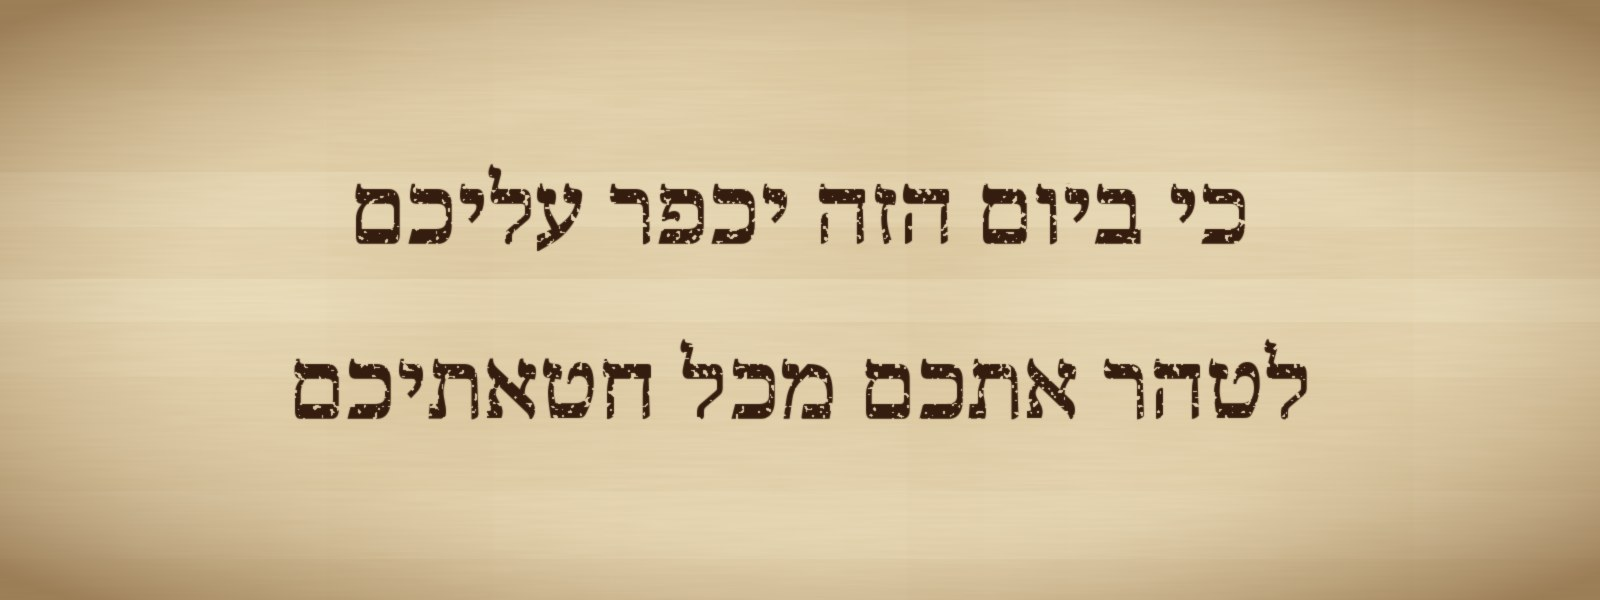
\includegraphics[width=0.78\linewidth,height=0.34\textheight,keepaspectratio]{portada.jpg}\\[-1pt]
  {\fontsize{5}{6}\selectfont\color{sepia}\textit{Nota.} Elaboración propia: Lv 16:30a en texto hebreo consonántico (BHS).}}
\begin{document}
\frame{\titlepage}

\begin{frame}\frametitle{Contenidos}
\begin{columns}[t,onlytextwidth]
\begin{column}{0.48\textwidth}\tableofcontents[sections={1-7}]\end{column}
\begin{column}{0.48\textwidth}\tableofcontents[sections={8-14}]\end{column}
\end{columns}
\end{frame}

% ==================================================================
\section{Introducción}

\begin{frame}{Un Dios santo en medio de un pueblo impuro}
\begin{cita}\ldots{}de la misma manera hará también al tabernáculo de reunión, el cual reside entre ellos en medio de sus impurezas.\fuente{(Lv 16:16, RVR1960)}\end{cita}
\small
\begin{itemize}
\item El pecado alcanza más allá de la conciencia: \destacar{mancha el lugar donde Dios habita}.
\item Dios decide quedarse con un pueblo impuro, y para ello prescribe \destacar{un día en que su morada sea limpiada}.
\item \heb{יוֹם הַכִּפֻּרִים} (\emph{Yom haKipurim}, Lv 23:27): ``el día de las expiaciones''. Sexta convocación, la única con \destacar{ayuno}, y el único día en que un hombre cruza el velo.
\end{itemize}
\end{frame}

\begin{frame}{El ciclo de Levítico 23}
\centering
\resizebox{\linewidth}{!}{%
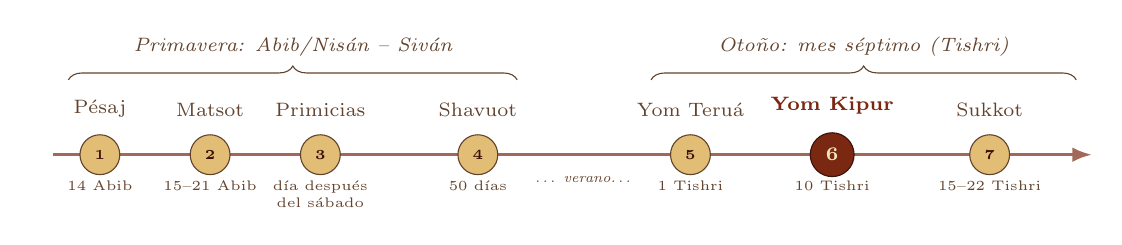
\begin{tikzpicture}[x=1cm,y=1cm,font=\scriptsize]
 \def\fiestaactual{6}
 \draw[line width=1.2pt,tierraroja!70,-{Latex[length=2.5mm]}] (0,0) -- (13.2,0);
 \draw[decorate,decoration={brace,amplitude=5pt},sepia] (0.2,0.95) -- (5.9,0.95) node[midway,above=5pt,font=\scriptsize\itshape]{Primavera: Abib/Nisán -- Siván};
 \draw[decorate,decoration={brace,amplitude=5pt},sepia] (7.6,0.95) -- (13.0,0.95) node[midway,above=5pt,font=\scriptsize\itshape]{Otoño: mes séptimo (Tishri)};
 \foreach \n/\x/\t/\d in {1/0.6/Pésaj/{14 Abib},2/2.0/Matsot/{15--21 Abib},3/3.4/Primicias/{día después del sábado},4/5.4/Shavuot/{50 días},5/8.1/Yom Teruá/{1 Tishri},6/9.9/Yom Kipur/{10 Tishri},7/11.9/Sukkot/{15--22 Tishri}}{
   \ifnum\n=\fiestaactual
     \node[circle,fill=tierraroja,draw=caferojizo,minimum size=5.5mm,text=papiro,font=\scriptsize\bfseries] at (\x,0) {\n};
     \node[above=3pt,font=\scriptsize\bfseries,text=tierraroja] at (\x,0.28) {\t};
   \else
     \node[circle,fill=mostaza!70,draw=sepia,minimum size=4.5mm,text=caferojizo,font=\tiny\bfseries] at (\x,0) {\n};
     \node[above=3pt,text=sepia] at (\x,0.25) {\t};
   \fi
   \node[below=6pt,text width=1.6cm,align=center,font=\tiny,text=sepia] at (\x,0) {\d};}
 \node[font=\tiny\itshape,text=sepia] at (6.75,-0.32) {\ldots\ verano\ldots};
\end{tikzpicture}}\par\medskip
\small\RaggedRight Entre el \destacar{sonido de trompeta} (1 Tishri) y la alegría de \destacar{las cabañas} (15 Tishri), el pueblo se detiene, ayuna y es declarado limpio. ``Afligiréis vuestras almas'' (Lv 16:29; 23:27).
\end{frame}

\begin{frame}{Los nombres del día}
\scriptsize\renewcommand{\arraystretch}{1.18}
\begin{tabular}{@{}L{3.0cm}L{5.0cm}L{3.4cm}@{}}
\toprule
\textbf{Nombre} & \textbf{Fundamento} & \textbf{Fuente} \\ \midrule
Día de las expiaciones & \heb{יוֹם הַכִּפֻּרִים}, Lv 23:27--28; 25:9 & bíblica \\
Reposo solemne & \heb{שַׁבַּת שַׁבָּתוֹן}, Lv 16:31; 23:32 & bíblica \\
El Ayuno & \grc{ἡ νηστεία}, Hch 27:9; Filón & NT y judaísmo helenista \\
El Día & \emph{Yomá}, tratado de la Misná & rabínica \\
Cara a cara & ante la \emph{kapóret} (Lv 16:2); cf. 1~Co 13:12 & lectura devocional \\
El gran shofar & shofar del Jubileo en Yom Kipur (Lv 25:9) & bíblica; Is 27:13 es interpretación \\
Cierre de las puertas & \emph{Neilá}, oración final & litúrgica posterior \\
\bottomrule
\end{tabular}\par\medskip
\precision{nombres recogidos en mis presentaciones anteriores; se distingue lo bíblico de lo tradicional.}
\end{frame}

\begin{frame}{Tesis y ruta}
\begin{tcolorbox}[colback=papiro,colframe=tierraroja,boxrule=1.2pt,arc=3pt]
\centering\small\itshape Yom Kipur es el día en que Dios purifica su morada para seguir habitando con su pueblo. La sangre limpia de dentro hacia fuera, y el macho vivo se lleva las culpas lejos.
\end{tcolorbox}
\centering
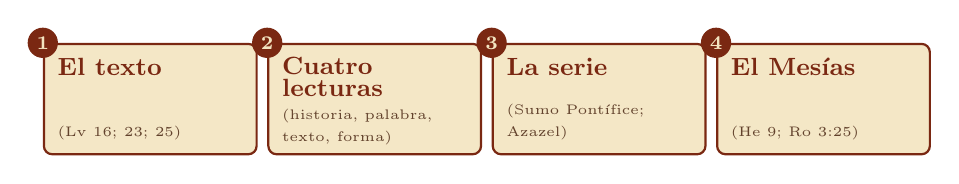
\begin{tikzpicture}
 \foreach \x/\n/\t/\r in {0/1/{El texto}/{Lv 16; 23; 25}, 2.85/2/{Cuatro lecturas}/{historia, palabra, texto, forma}, 5.7/3/{La serie}/{Sumo Pontífice; Azazel}, 8.55/4/{El Mesías}/{He 9; Ro 3:25}}{
  \node[caja,anchor=north] (b\n) at (\x,0) {\parbox[t][1.05cm][t]{2.35cm}{\RaggedRight
    {\small\textbf{\textcolor{tierraroja}{\t}}}\par\vfill{\tiny\color{sepia}(\r)}}};
  \node[circle,fill=tierraroja,text=papiro,font=\scriptsize\bfseries,inner sep=1.6pt] at (b\n.north west) {\n};}
\end{tikzpicture}
\end{frame}

% ==================================================================
\section{El texto}

\begin{frame}{Después de Nadab y Abiú}
\begin{columns}[t,onlytextwidth]
\begin{column}{0.52\textwidth}
\begin{cita}\ldots{}ofrecieron delante de \SENOR{} fuego extraño, que él nunca les mandó. Y salió fuego de delante de \SENOR{} y los quemó\ldots{} En los que a mí se acercan me santificaré.\fuente{(Lv 10:1--3)}\end{cita}
\end{column}
\begin{column}{0.46\textwidth}
\begin{cita}Di a Aarón tu hermano, que no en todo tiempo entre en el santuario detrás del velo\ldots{} para que no muera; porque yo apareceré en la nube sobre el propiciatorio.\fuente{(Lv 16:2)}\end{cita}
\end{column}
\end{columns}
\small\RaggedRight El verbo \heb{קָרַב} (\emph{qarav}, ``acercarse'') une ambos textos (16:1; 10:3). La pregunta que plantea el texto: \destacar{¿cómo entra un pecador ante Dios y sale vivo?} De la restricción ``no en todo tiempo'' nace el día.
\end{frame}

\begin{frame}{Texto ancla: Lv 16:30}
\fotolado{panel_lv16_30.jpg}{Elaboración propia: Lv 16:30 en texto hebreo consonántico (BHS).}
\begin{columns}[c,onlytextwidth]
\begin{column}{0.57\textwidth}
\begin{cita}Porque en este día se hará expiación por vosotros, y seréis limpios de todos vuestros pecados delante de \SENOR. Día de reposo es para vosotros, y afligiréis vuestras almas; es estatuto perpetuo.\fuente{(Lv 16:30--31)}\end{cita}
\small El versículo termina con un verbo: \heb{תִּטְהָרוּ} (\emph{titharu}), \destacar{``seréis puros''}. Todo el aparato de sangre, incienso y suertes apunta a la pureza del pueblo ``delante de \SENOR''.
\end{column}
\begin{column}{0.41\textwidth}\end{column}
\end{columns}
\end{frame}

\begin{frame}{Las vestiduras de lino}
\begin{columns}[c,onlytextwidth]
\begin{column}{0.55\textwidth}
\begin{cita}Se vestirá la túnica santa de lino, y sobre su cuerpo tendrá calzoncillos de lino, y se ceñirá el cinto de lino, y con la mitra de lino se cubrirá. Son las santas vestiduras\ldots\fuente{(Lv 16:4)}\end{cita}
\end{column}
\begin{column}{0.43\textwidth}\small
\begin{itemize}
\item Cuatro veces \heb{בַּד} (\emph{bad}, ``lino''): la ropa de los ángeles (Ez 9:2; Dn 10:5).
\item Distintas de las vestiduras ``para honra y hermosura'' (Éx 28:2): el sumo sacerdote entra como \destacar{siervo}.
\end{itemize}
\end{column}
\end{columns}
\precision{el efod, el pectoral con las doce tribus y la lámina ``Santidad a \SENOR'' (que figuran en mis láminas) son bíblicos (Éx 28), pero en el rito interior se usaba lino; el oro se vestía después, para los holocaustos (Lv 16:23--24). Las cinco inmersiones son práctica del Segundo Templo (Misná Yomá 3:3).}
\end{frame}

\begin{frame}{Las suertes: Lv 16:8}
\fotolado{panel_lv16_8.jpg}{Elaboración propia: Lv 16:8 en texto hebreo consonántico (BHS).}
\begin{columns}[c,onlytextwidth]
\begin{column}{0.57\textwidth}
\begin{cita}Y echará suertes Aarón sobre los dos machos cabríos; una suerte por \SENOR, y otra suerte por Azazel.\fuente{(Lv 16:8)}\end{cita}
\small
\begin{itemize}
\item \heb{לַיהוָה} / \heb{לַעֲזָאזֵל}: dos términos en \destacar{construcción paralela}.
\item \heb{גּוֹרָל} (\emph{goral}): Dios decide la función de cada animal (cf. Pr 16:33).
\item El del \SENOR{} se ofrece; el de Azazel se presenta \destacar{vivo} ``delante de \SENOR'' (v. 10).
\end{itemize}
\end{column}
\begin{column}{0.41\textwidth}\end{column}
\end{columns}
\end{frame}

\begin{frame}{El rito paso a paso}
\centering
\resizebox{\linewidth}{!}{%
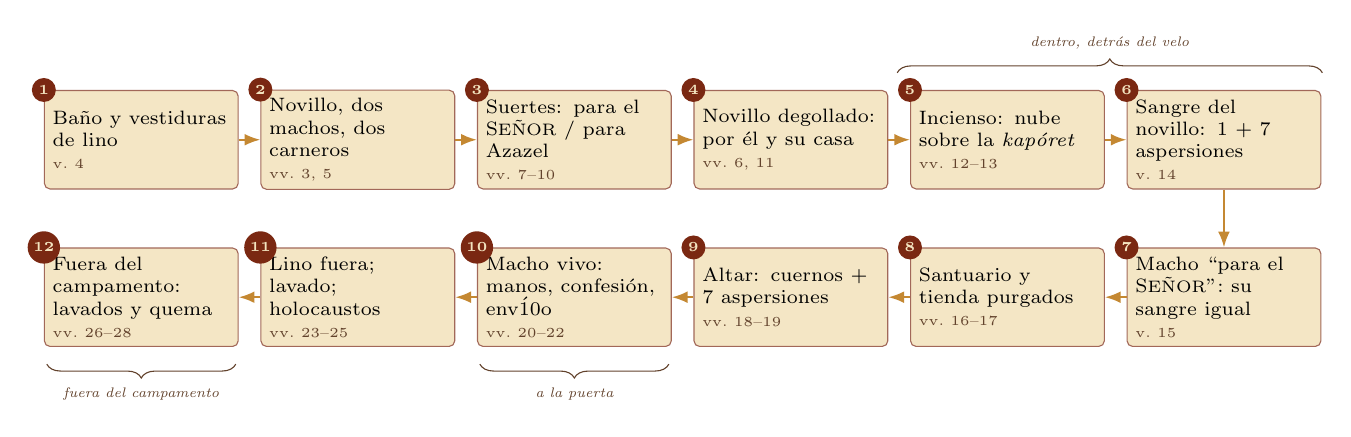
\begin{tikzpicture}[font=\scriptsize,
  paso/.style={draw=tierraroja!70,fill=papiro,fill opacity=0.92,text opacity=1,rounded corners=2pt,text width=2.25cm,minimum height=1.25cm,align=left,inner sep=3pt},
  num/.style={circle,fill=tierraroja,text=papiro,font=\tiny\bfseries,inner sep=1.3pt},
  fl/.style={-{Latex[length=2mm]},mostaza!80!tierraroja,line width=0.8pt}]
 \foreach \i/\x/\y/\t/\r in {
  1/0/0/{Baño y vestiduras de lino}/{v.~4},
  2/2.75/0/{Novillo, dos machos, dos carneros}/{vv.~3, 5},
  3/5.5/0/{Suertes: para el \SENOR{} / para Azazel}/{vv.~7--10},
  4/8.25/0/{Novillo degollado: por él y su casa}/{vv.~6, 11},
  5/11.0/0/{Incienso: nube sobre la \emph{kapóret}}/{vv.~12--13},
  6/13.75/0/{Sangre del novillo: 1 + 7 aspersiones}/{v.~14},
  7/13.75/-2.0/{Macho ``para el \SENOR'': su sangre igual}/{v.~15},
  8/11.0/-2.0/{Santuario y tienda purgados}/{vv.~16--17},
  9/8.25/-2.0/{Altar: cuernos + 7 aspersiones}/{vv.~18--19},
  10/5.5/-2.0/{Macho vivo: manos, confesión, envío}/{vv.~20--22},
  11/2.75/-2.0/{Lino fuera; lavado; holocaustos}/{vv.~23--25},
  12/0/-2.0/{Fuera del campamento: lavados y quema}/{vv.~26--28}}{
  \node[paso] (p\i) at (\x,\y) {\RaggedRight \t\par{\tiny\color{sepia}\r}};
  \node[num] at (p\i.north west) {\i};}
 \foreach \a/\b in {1/2,2/3,3/4,4/5,5/6,7/8,8/9,9/10,10/11,11/12} \draw[fl] (p\a) -- (p\b);
 \draw[fl] (p6) -- (p7);
 \draw[decorate,decoration={brace,amplitude=5pt},sepia] (9.6,0.85) -- (15.0,0.85) node[midway,above=5pt,font=\tiny\itshape]{dentro, detrás del velo};
 \draw[decorate,decoration={brace,amplitude=5pt,mirror},sepia] (4.3,-2.85) -- (6.7,-2.85) node[midway,below=5pt,font=\tiny\itshape]{a la puerta};
 \draw[decorate,decoration={brace,amplitude=5pt,mirror},sepia] (-1.2,-2.85) -- (1.2,-2.85) node[midway,below=5pt,font=\tiny\itshape]{fuera del campamento};
\end{tikzpicture}}\par\medskip
{\fontsize{5}{6}\selectfont\color{sepia}\textit{Nota.} Elaboración propia sobre Lv 16 (RVR1960).}
\end{frame}

\begin{frame}{La confesión: Lv 16:21}
\fotolado{panel_lv16_21.jpg}{Elaboración propia: Lv 16:21 (parte) en texto hebreo consonántico (BHS).}
\begin{columns}[c,onlytextwidth]
\begin{column}{0.57\textwidth}
\begin{cita}\ldots{}y pondrá Aarón sus dos manos sobre la cabeza del macho cabrío vivo, y confesará sobre él todas las iniquidades de los hijos de Israel, todas sus rebeliones y todos sus pecados, poniéndolos así sobre la cabeza del macho cabrío, y lo enviará al desierto por mano de un hombre destinado para esto.\fuente{(Lv 16:21)}\end{cita}
\scriptsize Es el único rito con \destacar{dos manos} y confesión sobre un animal. Al macho no se lo sacrifica: se lo \emph{envía} (\heb{שִׁלַּח}, vv. 10, 21, 22).
\end{column}
\begin{column}{0.41\textwidth}\end{column}
\end{columns}
\end{frame}

\begin{frame}{Lv 23:26--32: el día del pueblo}
\begin{columns}[t,onlytextwidth]
\begin{column}{0.54\textwidth}
\begin{cita}Porque toda persona que no se afligiere en este mismo día, será cortada de su pueblo\ldots{} comenzando a los nueve días del mes en la tarde; de tarde a tarde guardaréis vuestro reposo.\fuente{(Lv 23:29, 32)}\end{cita}
\end{column}
\begin{column}{0.44\textwidth}\small
\begin{itemize}
\item Única convocación con \destacar{\emph{karet}} (v. 29) y ``yo destruiré'' (v. 30).
\item Tres veces \heb{בְּעֶצֶם הַיּוֹם הַזֶּה}, ``en este mismo día''.
\item Fija el cómputo: \destacar{de tarde a tarde} (v. 32).
\end{itemize}
\end{column}
\end{columns}
\end{frame}

\begin{frame}{Tabla sinóptica}
\scriptsize\renewcommand{\arraystretch}{1.2}
\begin{tabular}{@{}L{1.7cm}L{3.0cm}L{6.8cm}@{}}
\toprule
\textbf{Texto} & \textbf{Perspectiva} & \textbf{Qué añade} \\ \midrule
Éx 30:10 & altar del incienso & expiación anual sobre sus cuernos (\emph{jatat hakipurim}) \\
Lv 16:1--28 & santuario & velo, lino, suertes, sangre sobre la \emph{kapóret}, macho vivo, lavados \\
Lv 16:29--34 & calendario & 10 del mes 7; afligir el alma; \emph{shabat shabatón}; natural y extranjero; ``una vez al año'' \\
Lv 23:26--32 & pueblo convocado & \emph{mikrá kódesh}; \emph{karet}; ``de tarde a tarde'' \\
Lv 25:8--10 & ciclo de años & el shofar del año 50 suena en Yom Kipur; \emph{derór} \\
Nm 29:7--11 & ofrendas & 1 becerro, 1 carnero, 7 corderos; \emph{jatat} adicional \\
\bottomrule
\end{tabular}\par\medskip
\precision{Dt 16, que legisla las fiestas de peregrinación, no menciona el día: el pueblo ayuna ``en dondequiera que habitéis'' (Lv 23:31).}
\end{frame}

% ==================================================================
\section{Historia}

\begin{frame}{El mes séptimo y el Cercano Oriente}
\begin{columns}[t,onlytextwidth]
\begin{column}{0.49\textwidth}\small
\destacar{El año agrícola}
\begin{itemize}
\item Fines de septiembre: cosecha guardada, se esperan las primeras lluvias.
\item ``Por haber pasado ya el ayuno'', la navegación era peligrosa (Hch 27:9).
\end{itemize}
\end{column}
\begin{column}{0.49\textwidth}\small
\destacar{Ritos de eliminación}
\begin{itemize}
\item Hititas: animal enviado al territorio enemigo con el mal.
\item Babilonia (\emph{akītu}): templo de Nabû ``frotado'' (\emph{kuppuru}) con un carnero arrojado al río.
\item En Lv 16 no hay magia: lo que se elimina son \destacar{pecados confesados} (Wright, 1987; Milgrom, 1991).
\end{itemize}
\end{column}
\end{columns}
\end{frame}

\begin{frame}{El día en las fuentes}
\centering
\resizebox{\linewidth}{!}{%
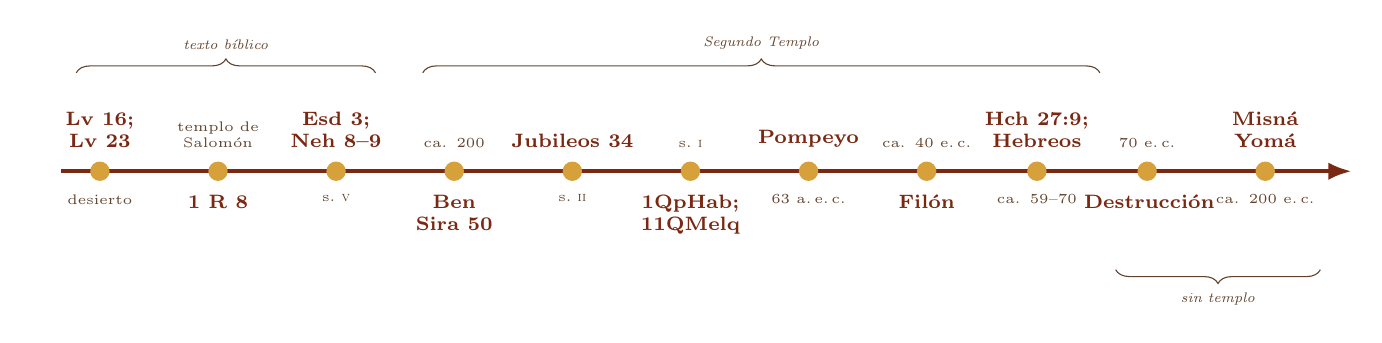
\begin{tikzpicture}[font=\scriptsize]
 \draw[line width=1.6pt,tierraroja,-{Latex[length=3mm]}] (0,0) -- (16.4,0);
 \foreach \x/\a/\b/\s in {
   0.5/{Lv 16; Lv 23}/{desierto}/1, 2.0/{1 R 8}/{templo de Salomón}/-1, 3.5/{Esd 3; Neh 8--9}/{s.~\textsc{v}}/1,
   5.0/{Ben Sira 50}/{ca. 200}/-1, 6.5/{Jubileos 34}/{s.~\textsc{ii}}/1, 8.0/{1QpHab; 11QMelq}/{s.~\textsc{i}}/-1,
   9.5/{Pompeyo}/{63 a.\,e.\,c.}/1, 11.0/{Filón}/{ca. 40 e.\,c.}/-1, 12.4/{Hch 27:9; Hebreos}/{ca. 59--70}/1,
   13.8/{Destrucción}/{70 e.\,c.}/-1, 15.3/{Misná Yomá}/{ca. 200 e.\,c.}/1}{
   \fill[mostaza] (\x,0) circle (3.5pt);
   \ifnum\s=1
     \node[above=5pt,font=\scriptsize\bfseries,text=tierraroja,text width=1.6cm,align=center] at (\x,0) {\a};
     \node[below=5pt,text width=1.6cm,align=center,font=\tiny,text=sepia] at (\x,0) {\b};
   \else
     \node[below=5pt,font=\scriptsize\bfseries,text=tierraroja,text width=1.6cm,align=center] at (\x,0) {\a};
     \node[above=5pt,text width=1.6cm,align=center,font=\tiny,text=sepia] at (\x,0) {\b};
   \fi}
 \draw[decorate,decoration={brace,amplitude=5pt},sepia] (0.2,1.25) -- (4.0,1.25) node[midway,above=5pt,font=\tiny\itshape]{texto bíblico};
 \draw[decorate,decoration={brace,amplitude=5pt},sepia] (4.6,1.25) -- (13.2,1.25) node[midway,above=5pt,font=\tiny\itshape]{Segundo Templo};
 \draw[decorate,decoration={brace,amplitude=5pt,mirror},sepia] (13.4,-1.25) -- (16.0,-1.25) node[midway,below=5pt,font=\tiny\itshape]{sin templo};
\end{tikzpicture}}\par\medskip
\small\RaggedRight Ningún libro histórico narra un Yom Kipur: en Neh 9:1 el ayuno cae el día 24, y la tradición discute si Salomón ayunó (b. Moed Katán 9a).
\end{frame}

\begin{frame}{La salida del sumo sacerdote}
\begin{columns}[c,onlytextwidth]
\begin{column}{0.52\textwidth}
\begin{cita}¡Qué glorioso era\ldots{} cuando salía de la casa del velo! Como la estrella de la mañana entre las nubes\ldots\fuente{(Si 50:5--6, trad. propia)}\end{cita}
\small \grc{ἐν ἐξόδῳ οἴκου καταπετάσματος}: la \destacar{alegría de verlo salir vivo}.
\end{column}
\begin{column}{0.46\textwidth}\small
\destacar{Jubileos 34:12--19}: el día recuerda el cabrito con cuya sangre los hijos de Jacob mancharon la túnica de José. Una \emph{lectura memorial} antigua.\par\medskip
\precision{para algunos, Si 50 describe el sacrificio diario (\emph{tamid}) y no Yom Kipur (Hayward, 1996).}
\end{column}
\end{columns}
\end{frame}

\begin{frame}{Qumrán, Filón y Josefo}
\begin{cita}\ldots{}y en el tiempo de la fiesta del reposo del Día de las Expiaciones se les apareció para devorarlos y hacerlos tropezar en el día de ayuno, sábado de su reposo.\fuente{(1QpHab XI 6--8; trad. según García Martínez, 1992)}\end{cita}
\scriptsize
\begin{itemize}
\item El Sacerdote Impío ataca al Maestro de Justicia en \emph{su} Yom Kipur: indicio de \destacar{calendarios distintos} (VanderKam, 1998).
\item Filón: ``el Ayuno'', fiesta sin comida en que el alma se nutre de oración (\emph{Spec.} 1.186--188; 2.193--203).
\item Josefo: el macho enviado al desierto como expiación (\emph{Ant.} 3.240--243); Pompeyo toma el templo ``el día del ayuno'' (14.66).
\end{itemize}
\end{frame}

\begin{frame}{La destrucción del año 70}
\begin{columns}[t,onlytextwidth]
\begin{column}{0.50\textwidth}\small
Sin templo desaparecen el sumo sacerdote y el macho para Azazel; el día sobrevive como \destacar{ayuno, oración y confesión}.\par\medskip
En mis láminas destaqué que, ``cuarenta años antes de la destrucción'', la cinta escarlata \destacar{no se volvió blanca}.
\end{column}
\begin{column}{0.48\textwidth}
\begin{tcolorbox}[colback=mostaza!12,colframe=mostaza!80!tierraroja,boxrule=0.6pt,arc=2pt,fontupper=\scriptsize,title={\scriptsize Precisión},coltitle=caferojizo,colbacktitle=mostaza!35]
La noticia no está en la Misná: es una \emph{baraita} del Talmud (b. Yomá 39b): la suerte no salía en la derecha, la cinta no blanqueaba, la lámpara occidental se apagaba, las puertas se abrían solas. La conexión con la cruz es lectura cristiana.
\end{tcolorbox}
\end{column}
\end{columns}
\end{frame}

% ==================================================================
\section{Filología}

\begin{frame}{\heb{כִּפֶּר} (\emph{kipper}): tres caras}
\centering
\begin{tikzpicture}[font=\scriptsize]
 \node[draw=tierraroja,line width=1pt,fill=papiro,rounded corners=3pt,inner sep=6pt,align=center] (k) at (0,0) {\large\heb{כִּפֶּר}\\ \emph{kipper}\\ \tiny 16 veces en Lv 16};
 \node[caja,text width=3.1cm,align=left] (a) at (-4.2,-1.6) {\textbf{\textcolor{tierraroja}{Cubrir}}\\ \heb{וְכָפַרְתָּ} ``la calafatearás'' (Gn 6:14)};
 \node[caja,text width=3.1cm,align=left] (b) at (0,-1.9) {\textbf{\textcolor{tierraroja}{Rescatar}}\\ \heb{כֹּפֶר} ``rescate'' (Éx 21:30; 30:12, 16)};
 \node[caja,text width=3.1cm,align=left] (c) at (4.2,-1.6) {\textbf{\textcolor{tierraroja}{Purgar}}\\ acadio \emph{kuppuru}; Milgrom (1991); Levine (1989)};
 \foreach \n in {a,b,c}\draw[-{Latex[length=2mm]},mostaza!80!tierraroja,line width=0.9pt] (k) -- (\n);
\end{tikzpicture}\par\medskip
\scriptsize\RaggedRight Sintaxis: \heb{כִּפֶּר אֶת־הַקֹּדֶשׁ} ``expiar el santuario'' (cosas, vv. 20, 33); \heb{בְּעַד} ``a favor de'' (personas, vv. 6, 11, 17, 24). LXX: \grc{ἐξιλάσκομαι}.\par
\precision{Gane (2005): la \emph{jatat} del año purifica al oferente; en Yom Kipur Dios purga su morada de las faltas ya perdonadas.}
\end{frame}

\begin{frame}{\emph{Kipurim} y \emph{kapóret}}
\begin{columns}[t,onlytextwidth]
\begin{column}{0.49\textwidth}\small
\destacar{\heb{כִּפֻּרִים} \emph{kipurim}}
\begin{itemize}
\item Plural abstracto e intensivo: la expiación plena (como \emph{bikurim}).
\item 8 veces, siempre en plural (Éx 29:36; 30:10, 16; Lv 23:27--28; 25:9; Nm 5:8; 29:11).
\item LXX \grc{ἡμέρα ἐξιλασμοῦ}.
\end{itemize}
\end{column}
\begin{column}{0.49\textwidth}\small
\destacar{\heb{כַּפֹּרֶת} \emph{kapóret}}
\begin{itemize}
\item La tapa del arca, lugar del \destacar{encuentro} (Éx 25:22).
\item 27 veces; \destacar{7 en Lv 16}.
\item LXX \grc{ἱλαστήριον}; Vulgata \emph{propitiatorium}; He 9:5; Ro 3:25.
\end{itemize}
\end{column}
\end{columns}\par\medskip
\precision{conteos propios por lema sobre el Códice de Leningrado.}
\end{frame}

\begin{frame}{Las tres palabras del pecado}
\centering
\resizebox{0.95\linewidth}{!}{%
\begin{tikzpicture}[font=\small,
  pal/.style={draw=tierraroja!70,fill=papiro,fill opacity=0.92,text opacity=1,rounded corners=3pt,text width=3.4cm,align=center,inner sep=4pt},
  fl/.style={-{Latex[length=2mm]},mostaza!80!tierraroja,line width=0.9pt}]
 \node[pal] (a) at (0,2.3) {\heb{עֲוֺנֹת} \emph{avonot}\\ \footnotesize ``iniquidades''\\ \scriptsize\color{sepia} torcer: culpa que pesa};
 \node[pal] (p) at (4.8,2.3) {\heb{פְּשָׁעִים} \emph{peshaím}\\ \footnotesize ``rebeliones''\\ \scriptsize\color{sepia} romper la lealtad};
 \node[pal] (j) at (9.6,2.3) {\heb{חַטֹּאת} \emph{jatot}\\ \footnotesize ``pecados''\\ \scriptsize\color{sepia} errar el blanco (Jue 20:16)};
 \node[draw=tierraroja,line width=0.9pt,fill=tierraroja!8,rounded corners=3pt,text width=7.4cm,align=center,inner sep=5pt] (c) at (4.8,0.0)
   {\heb{וְהִתְוַדָּה עָלָיו}\\ ``confesará sobre él'' (Lv 16:21)};
 \node[pal,text width=7.4cm] (d) at (4.8,-1.9) {\heb{וְנָשָׂא הַשָּׂעִיר עָלָיו}\\ ``llevará sobre sí\ldots{} a tierra inhabitada'' (Lv 16:22)};
 \draw[fl] (a) -- (c); \draw[fl] (p) -- (c); \draw[fl] (j) -- (c); \draw[fl] (c) -- (d);
\end{tikzpicture}}\par\smallskip
\scriptsize La misma tríada en el Nombre: Dios ``perdona la iniquidad, la rebelión y el pecado'' (Éx 34:7). \emph{Pésha} solo aparece en Levítico en 16:16, 21.
\end{frame}

\begin{frame}{\heb{נָשָׂא עָוֺן} (\emph{nasá avón}): llevar la iniquidad}
\begin{columns}[t,onlytextwidth]
\begin{column}{0.49\textwidth}\small
\destacar{Cargar la culpa propia}
\begin{itemize}
\item ``llevaréis vuestras iniquidades cuarenta años'' (Nm 14:34).
\item Lv 5:1, 17.
\end{itemize}
\destacar{Quitar la culpa de otro}
\begin{itemize}
\item Dios \heb{נֹשֵׂא עָוֺן} (Éx 34:7; Nm 14:18; Mi 7:18).
\end{itemize}
\end{column}
\begin{column}{0.49\textwidth}\small
\destacar{El macho y el Siervo}
\begin{itemize}
\item ``aquel macho cabrío llevará sobre sí todas las iniquidades'' (Lv 16:22).
\item ``habiendo él llevado el pecado de muchos'' (Is 53:12); ``fue cortado'' \heb{נִגְזַר} (53:8; cf. \heb{גְּזֵרָה}).
\item He 9:28: \grc{ἀνενεγκεῖν ἁμαρτίας}.
\end{itemize}
\end{column}
\end{columns}
\end{frame}

\begin{frame}{\heb{עֲזָאזֵל} (Azazel): cuatro hipótesis}
\scriptsize\renewcommand{\arraystretch}{1.18}
\begin{tabular}{@{}L{2.9cm}L{4.6cm}L{4.0cm}@{}}
\toprule
\textbf{Hipótesis} & \textbf{Base} & \textbf{Testigos} \\ \midrule
``El macho que se va'' & \heb{עֵז אֹזֵל} \emph{ez ozel} & LXX \grc{ἀποπομπαῖος}; Vulgata \emph{caper emissarius}; Tyndale \emph{scapegoat} \\
Lugar escarpado & ``el más duro de los montes'' & b. Yomá 67b; Targum Ps.-Jonatán; Misná Yomá 6; Driver (1956) \\
Ser demoníaco & paralelo \emph{laYHWH} / \emph{laAzazel} & 1~Enoc 8:1; 10:4--8; Milgrom; Levine; Hartley \\
Remoción total & raíz \emph{azal}, ``quitar'' & Brown, Driver y Briggs (1906) \\
\bottomrule
\end{tabular}\par\medskip
\small Solo 4 veces, todas en Lv 16 (vv. 8, 10, 10, 26). Los machos son \heb{שְׂעִירִם} (\emph{se'irim}); Lv 17:7 prohíbe sacrificar ``a los demonios'', también \emph{se'irim}.
\end{frame}

\begin{frame}{Afligir el alma; reposo absoluto}
\begin{columns}[t,onlytextwidth]
\begin{column}{0.49\textwidth}\small
\destacar{\heb{וְעִנִּיתֶם אֶת־נַפְשֹׁתֵיכֶם}}
\begin{itemize}
\item \emph{Néfesh}: garganta, apetito (Sal 107:9).
\item ``afligí con ayuno mi alma'' (Sal 35:13); Is 58:3; Esd 8:21.
\item = \destacar{ayuno}, de puesta a puesta de sol.
\end{itemize}
\end{column}
\begin{column}{0.49\textwidth}\small
\destacar{\heb{שַׁבַּת שַׁבָּתוֹן}}
\begin{itemize}
\item Superlativo: ``reposo de reposo''.
\item Solo: sábado, Yom Kipur, año sabático (Éx 31:15; Lv 16:31; 25:4).
\item ``ningún trabajo'' (\heb{כָּל־מְלָאכָה}), no solo ``obra de siervos''.
\end{itemize}
\end{column}
\end{columns}\par\medskip
\precision{las cinco abstenciones (comer y beber, lavarse, ungirse, sandalias, relaciones) son precisión rabínica (Misná Yomá 8:1).}
\end{frame}

\begin{frame}{Del hebreo al griego}
\centering
\resizebox{\linewidth}{!}{%
\begin{tikzpicture}[font=\small,
  cad/.style={draw=tierraroja!70,fill=papiro,fill opacity=0.92,text opacity=1,rounded corners=3pt,text width=3.2cm,align=center,inner sep=5pt,minimum height=2.3cm},
  fl/.style={-{Latex[length=2.2mm]},mostaza!80!tierraroja,line width=1pt}]
 \node[cad] (h) at (0,0) {\textbf{Hebreo}\\[2pt] \heb{כִּפֶּר} \emph{kipper}\\ \heb{כִּפֻּרִים} \emph{kipurim}\\ \heb{כַּפֹּרֶת} \emph{kapóret}};
 \node[cad] (s) at (4.1,0) {\textbf{Septuaginta}\\[2pt] \grc{ἐξιλάσκομαι}\\ \grc{ἐξιλασμός}\\ \grc{ἱλαστήριον}};
 \node[cad] (n) at (8.2,0) {\textbf{Nuevo Testamento}\\[2pt] \grc{ἱλάσκεσθαι} (He 2:17)\\ \grc{ἱλασμός} (1~Jn 2:2)\\ \grc{ἱλαστήριον} (Ro 3:25)};
 \node[cad] (e) at (12.3,0) {\textbf{Español}\\[2pt] expiar\\ propiciación\\ propiciatorio};
 \draw[fl] (h) -- (s); \draw[fl] (s) -- (n); \draw[fl] (n) -- (e);
\end{tikzpicture}}\par\medskip
\small\RaggedRight La tapa del arca y la persona de Cristo reciben el mismo nombre, porque ambas son \destacar{el lugar donde Dios trata el pecado} para seguir habitando con su pueblo. \grc{ἀρχιερεύς}: 17 veces en Hebreos (RV1909: ``pontífice'').
\end{frame}

% ==================================================================
\section{Texto}

\begin{frame}{Azazel en la Septuaginta}
\scriptsize\renewcommand{\arraystretch}{1.18}
\begin{tabular}{@{}L{1.2cm}L{3.4cm}L{4.0cm}L{2.9cm}@{}}
\toprule
\textbf{Verso} & \textbf{TM} & \textbf{LXX} & \textbf{Lectura} \\ \midrule
16:8 & \heb{לַעֲזָאזֵל} & \grc{τῷ ἀποπομπαίῳ} & el enviado lejos \\
16:10 & \heb{לְשַׁלַּח אֹתוֹ לַעֲזָאזֵל} & \grc{εἰς τὴν ἀποπομπήν} & el envío \\
16:21 & \heb{אִישׁ עִתִּי} & \grc{ἀνθρώπου ἑτοίμου} & hombre preparado \\
16:22 & \heb{אֶרֶץ גְּזֵרָה} & \grc{γῆν ἄβατον} & tierra intransitable \\
16:26 & \heb{הַשָּׂעִיר לַעֲזָאזֵל} & \grc{εἰς ἄφεσιν} & para la liberación \\
\bottomrule
\end{tabular}\par\medskip
\small\RaggedRight La LXX no lee un demonio: lee \destacar{alejamiento}. \grc{ἄφεσις} es también el Jubileo (Lv 25:10) y el ``perdón'' del NT (Mt 26:28; Lc 4:18).\par
\precision{Lv 16:21: el texto consonántico dice \heb{ידו}; se lee \heb{יָדָיו}, ``sus (dos) manos''. LXX según Rahlfs-Hanhart.}
\end{frame}

\begin{frame}{Dn 9:24: \emph{lekaper avón}}
\begin{cita}Setenta semanas están determinadas sobre tu pueblo y sobre tu santa ciudad, para terminar la prevaricación, y poner fin al pecado, y expiar la iniquidad, para traer la justicia perdurable\ldots{} y ungir al Santo de los santos.\fuente{(Dn 9:24)}\end{cita}
\small Vuelven \emph{pésha}, \emph{jatat}, \emph{avón} con \heb{לְכַפֵּר}. El documento de referencia: el Mesías se sacrifica ``para expiar la iniquidad'' (Dn 9:24).\par\medskip
\precision{texto consonántico \heb{ולחתם חטאות} (``sellar los pecados''), leído \heb{וּלְהָתֵם חַטָּאת} (``poner fin al pecado''). Los cómputos de las 490 años (Ciro, Artajerjes; o Antíoco IV) son lecturas, no datos del texto.}
\end{frame}

\begin{frame}{Ro 3:25 y He 9:4}
\begin{columns}[t,onlytextwidth]
\begin{column}{0.52\textwidth}
\begin{cita}\ldots{}a quien Dios puso como propiciación por medio de la fe en su sangre\ldots\fuente{(Ro 3:25)}\end{cita}
\scriptsize
\begin{itemize}
\item \grc{ἱλαστήριον}: ¿la \emph{kapóret} (He 9:5) o ``medio de propiciación'' (4 Mac 17:22)? Dunn (1998); Moo (1996).
\item ¿Expiación o propiciación? Dodd (1935) vs. Morris (1955).
\end{itemize}
\end{column}
\begin{column}{0.46\textwidth}\scriptsize
\destacar{He 9:4: ``un incensario de oro''} dentro del lugar santísimo.
\begin{itemize}
\item El altar estaba \emph{delante} del velo (Éx 30:6).
\item Pero 1~R 6:22: ``el altar que pertenecía al santuario interior''.
\item Hebreos mira el tabernáculo \destacar{desde Yom Kipur} (Attridge, 1989; Lane, 1991).
\end{itemize}
\end{column}
\end{columns}
\end{frame}

% ==================================================================
\section{Literatura}

\begin{frame}{Lv 16 en el centro del libro}
\centering
\resizebox{0.95\linewidth}{!}{%
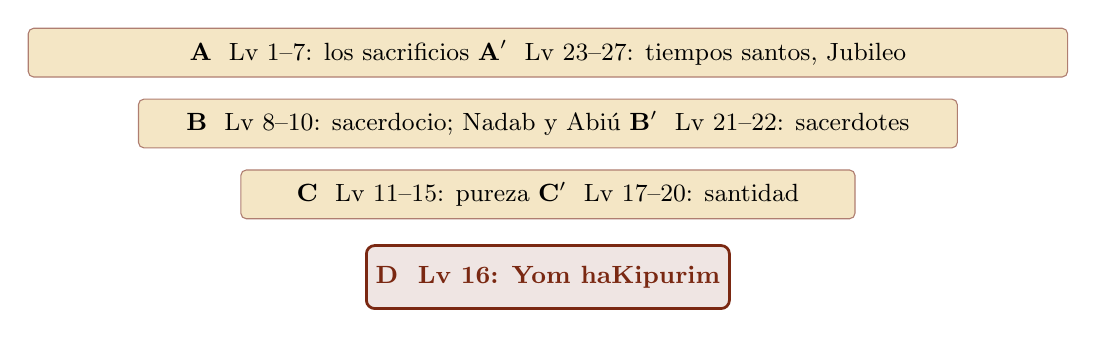
\begin{tikzpicture}[font=\small,x=1cm,y=1cm,
  bl/.style={draw=tierraroja!60,fill=papiro,fill opacity=0.92,text opacity=1,rounded corners=2pt,minimum height=0.62cm,align=center,inner sep=3pt}]
 \node[bl,minimum width=13.2cm] (a) at (0,3.0) {\textbf{A} \ Lv 1--7: los sacrificios \hfill \textbf{A$'$} \ Lv 23--27: tiempos santos, Jubileo};
 \node[bl,minimum width=10.4cm] (b) at (0,2.1) {\textbf{B} \ Lv 8--10: sacerdocio; Nadab y Abiú \hfill \textbf{B$'$} \ Lv 21--22: sacerdotes};
 \node[bl,minimum width=7.8cm] (c) at (0,1.2) {\textbf{C} \ Lv 11--15: pureza \hfill \textbf{C$'$} \ Lv 17--20: santidad};
 \node[draw=tierraroja,line width=1pt,fill=tierraroja!12,rounded corners=3pt,minimum width=4.6cm,minimum height=0.8cm,align=center,font=\small\bfseries,text=tierraroja] (d) at (0,0.15) {D \ Lv 16: Yom haKipurim};
\end{tikzpicture}}\par\medskip
\small\RaggedRight Lv 16:1 remite a Lv 10; limpia las impurezas de Lv 11--15; Lv 25:9 abre el Jubileo en Yom Kipur.\par
\precision{estructura concéntrica propuesta por varios autores (Douglas, 1999; Warning, 1999); otros sitúan el centro en Lv 19.}
\end{frame}

\begin{frame}{El recorrido: de dentro hacia fuera}
\centering
\resizebox{\linewidth}{!}{%
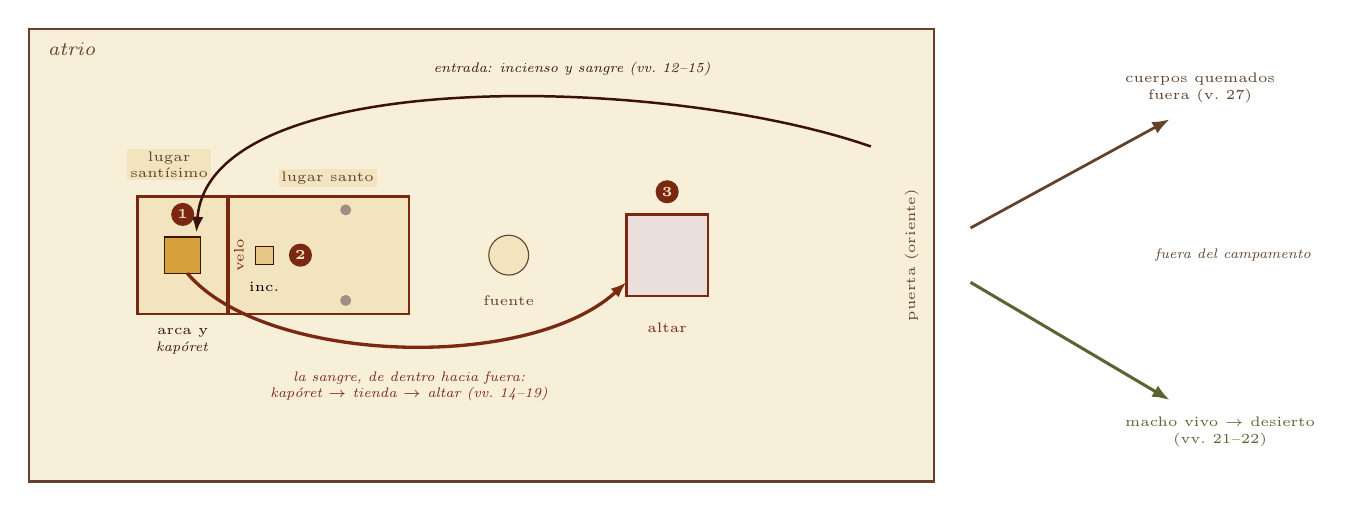
\begin{tikzpicture}[x=1.15cm,y=1.15cm,font=\scriptsize]
 \draw[sepia,line width=0.8pt,fill=papiro!60] (0,0) rectangle (10,5);
 \node[anchor=north west,text=sepia,font=\scriptsize\itshape] at (0.1,4.95) {atrio};
 \draw[tierraroja,line width=0.9pt,fill=papiro] (1.2,1.85) rectangle (4.2,3.15);
 \draw[tierraroja,line width=1.4pt] (2.2,1.85) -- (2.2,3.15);
 \node[text=tierraroja,font=\tiny,rotate=90] at (2.32,2.5) {velo};
 \node[text=sepia,font=\tiny,align=center,fill=papiro,inner sep=1pt] at (1.55,3.5) {lugar\\santísimo};
 \node[text=sepia,font=\tiny,align=center,fill=papiro,inner sep=1pt] at (3.3,3.35) {lugar santo};
 \draw[fill=mostaza,draw=caferojizo] (1.5,2.3) rectangle (1.9,2.7);
 \node[font=\tiny,text=caferojizo,align=center] at (1.7,1.55) {arca y\\\emph{kapóret}};
 \draw[fill=mostaza!60,draw=caferojizo] (2.5,2.4) rectangle (2.7,2.6);
 \node[font=\tiny] at (2.6,2.15) {inc.};
 \fill[sepia!60] (3.5,2.0) circle (2pt); \fill[sepia!60] (3.5,3.0) circle (2pt);
 \draw[sepia,fill=papiro] (5.3,2.5) circle (0.22);
 \node[font=\tiny,text=sepia] at (5.3,2.0) {fuente};
 \draw[tierraroja,fill=tierraroja!15,line width=0.8pt] (6.6,2.05) rectangle (7.5,2.95);
 \node[font=\tiny,text=tierraroja,align=center] at (7.05,1.7) {altar};
 \draw[sepia,line width=0.6pt,dashed] (10,1.9) -- (10,3.1);
 \node[font=\tiny,text=sepia,rotate=90] at (9.75,2.5) {puerta (oriente)};
 \draw[-{Latex[length=2mm]},caferojizo,line width=0.9pt] (9.3,3.7) .. controls (7,4.5) and (2.0,4.6) .. (1.85,2.75);
 \node[font=\tiny\itshape,text=caferojizo] at (6.0,4.55) {entrada: incienso y sangre (vv.~12--15)};
 \draw[-{Latex[length=2mm]},tierraroja,line width=1.2pt] (1.75,2.3) .. controls (2.6,1.3) and (5.5,1.2) .. (6.6,2.2);
 \node[font=\tiny\itshape,text=tierraroja,align=center] at (4.2,1.05) {la sangre, de dentro hacia fuera:\\kapóret $\rightarrow$ tienda $\rightarrow$ altar (vv.~14--19)};
 \foreach \x/\y/\n in {1.7/2.95/1, 3.0/2.5/2, 7.05/3.2/3}{\node[circle,fill=tierraroja,text=papiro,font=\tiny\bfseries,inner sep=1.2pt] at (\x,\y) {\n};}
 \draw[-{Latex[length=2.2mm]},oliva,line width=1.1pt] (10.4,2.2) -- (12.6,0.9);
 \node[font=\tiny,text=oliva,align=center,anchor=west] at (12.0,0.55) {macho vivo $\rightarrow$ desierto\\(vv.~21--22)};
 \draw[-{Latex[length=2.2mm]},sepia,line width=1pt] (10.4,2.8) -- (12.6,4.0);
 \node[font=\tiny,text=sepia,align=center,anchor=west] at (12.0,4.35) {cuerpos quemados\\fuera (v.~27)};
 \node[font=\tiny\itshape,text=sepia] at (13.3,2.5) {fuera del campamento};
\end{tikzpicture}}\par
{\fontsize{5}{6}\selectfont\color{sepia}\textit{Nota.} Elaboración propia sobre Éx 26--27; 30; Lv 16. 1 = \emph{kapóret} (1 + 7 aspersiones), 2 = tienda, 3 = altar (cuernos + 7).}\par\smallskip
\scriptsize\RaggedRight La purificación va \destacar{del centro a la periferia}, y la eliminación ocurre \destacar{fuera del todo}. Siete aspersiones tres veces; \emph{kapóret} 7 veces, \emph{jatat} 14 (conteo propio).
\end{frame}

\begin{frame}{Dos machos, un solo acto}
\centering
\resizebox{\linewidth}{!}{%
\begin{tikzpicture}[font=\small,
  hd/.style={font=\scriptsize\bfseries,text=sepia},
  bx/.style={draw=tierraroja!65,fill=papiro,fill opacity=0.92,text opacity=1,rounded corners=2pt,text width=3.55cm,align=center,inner sep=4pt,minimum height=1.25cm},
  fl/.style={-{Latex[length=2mm]},mostaza!80!tierraroja,line width=0.9pt}]
 \node[draw=tierraroja,line width=1pt,fill=tierraroja!10,rounded corners=3pt,text width=2.6cm,align=center,inner sep=5pt] (o) at (0,0) {Dos machos cabríos\\ \textbf{una} \emph{jatat}\\ \scriptsize (v.~5)};
 \node[hd] at (4.1,2.3) {Suerte}; \node[hd] at (8.2,2.3) {Destino}; \node[hd] at (12.3,2.3) {Sentido};
 \node[bx] (s1) at (4.1,1.1) {\heb{לַיהוָה}\\ ``para el \SENOR''};
 \node[bx] (d1) at (8.2,1.1) {degollado; su sangre ante y sobre la \emph{kapóret}};
 \node[bx] (m1) at (12.3,1.1) {purga el santuario (vv.~16--19)};
 \node[bx] (s2) at (4.1,-1.1) {\heb{לַעֲזָאזֵל}\\ ``para Azazel''};
 \node[bx] (d2) at (8.2,-1.1) {vivo; dos manos, confesión, envío};
 \node[bx] (m2) at (12.3,-1.1) {lleva las iniquidades ``a tierra cortada'' (v.~22)};
 \draw[fl] (o) -- (s1); \draw[fl] (o) -- (s2);
 \draw[fl] (s1) -- (d1); \draw[fl] (d1) -- (m1); \draw[fl] (s2) -- (d2); \draw[fl] (d2) -- (m2);
\end{tikzpicture}}\par\medskip
\small\RaggedRight Un paralelo que señalé en mis láminas: \destacar{las dos avecillas} (Lv 14:4--7). ``Soltará la avecilla viva\ldots{} Así hará expiación por la casa'' (Lv 14:53): también el animal que se suelta \emph{expía}.
\end{frame}

\begin{frame}{Ecos: Zacarías 3}
\begin{cita}Me mostró al sumo sacerdote Josué, el cual estaba delante del ángel de \SENOR, y Satanás estaba a su mano derecha para acusarle.\fuente{(Zac 3:1)}\end{cita}
\small
\begin{itemize}
\item ``Mira que he quitado de ti tu pecado, y te he hecho vestir de ropas de gala'' (3:4).
\item ``quitaré el pecado de la tierra \destacar{en un día}'' (3:9).
\item Sumo sacerdote, cambio de vestiduras, \destacar{acusador reprendido}: apoyo bíblico para leer el día como sentencia contra Satanás.
\end{itemize}
\scriptsize Otros ecos: Éx 32:30 (\heb{אֲכַפְּרָה}); Nm 14:20, 34; Is 53; Mi 7:19; Sal 103:12.
\end{frame}

\begin{frame}{El mes séptimo y el Jubileo}
\centering
\resizebox{\linewidth}{!}{%
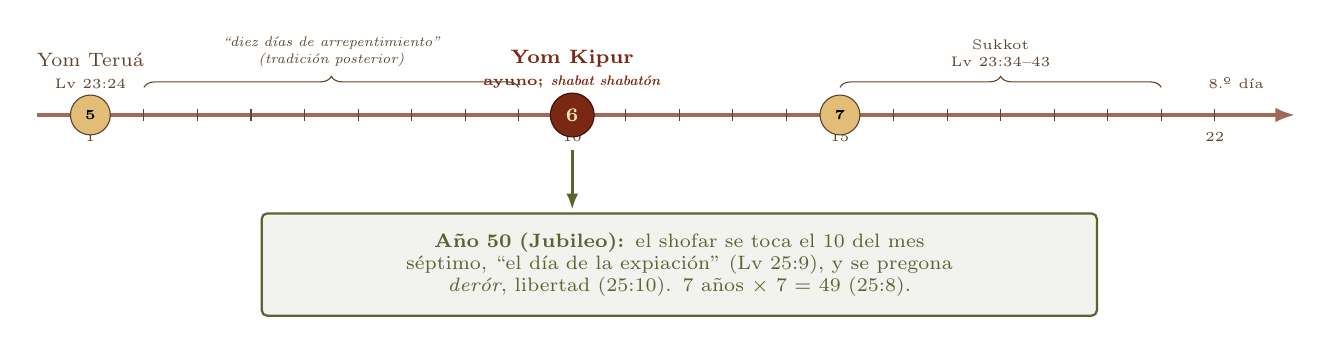
\begin{tikzpicture}[font=\scriptsize,x=0.68cm,y=1cm]
 \draw[line width=1.2pt,tierraroja!70,-{Latex[length=2.5mm]}] (0,0) -- (23.5,0);
 \foreach \d in {1,...,22}{\draw[sepia] (\d,-0.08) -- (\d,0.08);}
 \foreach \d in {1,10,15,22}{\node[below=3pt,font=\tiny,text=sepia] at (\d,0) {\d};}
 \node[circle,fill=mostaza!70,draw=sepia,minimum size=4.5mm,font=\tiny\bfseries] at (1,0) {5};
 \node[circle,fill=tierraroja,draw=caferojizo,minimum size=5.5mm,text=papiro,font=\scriptsize\bfseries] at (10,0) {6};
 \node[circle,fill=mostaza!70,draw=sepia,minimum size=4.5mm,font=\tiny\bfseries] at (15,0) {7};
 \node[above=6pt,text=sepia,align=center] at (1,0) {Yom Teruá\\ \tiny Lv 23:24};
 \node[above=6pt,text=tierraroja,font=\scriptsize\bfseries,align=center] at (10,0) {Yom Kipur\\ \tiny ayuno; \emph{shabat shabatón}};
 \draw[decorate,decoration={brace,amplitude=4pt},sepia] (2,0.35) -- (9,0.35) node[midway,above=4pt,font=\tiny\itshape,align=center]{``diez días de arrepentimiento''\\(tradición posterior)};
 \draw[decorate,decoration={brace,amplitude=4pt},sepia] (15,0.35) -- (21,0.35) node[midway,above=4pt,font=\tiny,align=center]{Sukkot\\ \tiny Lv 23:34--43};
 \node[above=6pt,text=sepia,align=center,font=\tiny] at (22.4,0) {8.º día};
 \draw[oliva,line width=0.8pt,rounded corners=2pt,fill=oliva!8] (4.2,-1.25) rectangle (19.8,-2.55);
 \node[text=oliva,font=\scriptsize,align=center,text width=10.2cm] at (12,-1.9) {\textbf{Año 50 (Jubileo):} el shofar se toca el 10 del mes séptimo, ``el día de la expiación'' (Lv 25:9), y se pregona \emph{derór}, libertad (25:10). 7 años $\times$ 7 = 49 (25:8).};
 \draw[-{Latex[length=2mm]},oliva,line width=0.9pt] (10,-0.45) -- (10,-1.2);
\end{tikzpicture}}\par\medskip
\small\RaggedRight El mismo día que limpia el santuario \destacar{libera la tierra y a los esclavos}. Is 61:1 (\emph{derór}) $\rightarrow$ Lc 4:18. Véase el estudio 09, \emph{El Jubileo}.
\end{frame}

% ==================================================================
\section{La serie}

\begin{frame}{Memorial: el fin del juicio}
\begin{cita}[fontupper=\scriptsize\itshape]\ldots{}esta era la más explícita señal de que, por fin había concluido el juicio de Dios a la nación; y les había sido concedido el perdón, tras las rebeliones en el desierto; particularmente aquella en que se negaron a entrar en la Tierra Prometida\ldots\fuente{(Documento de referencia, lección 8)}\end{cita}
\scriptsize\renewcommand{\arraystretch}{1.1}
\begin{tabular}{@{}L{3.5cm}L{2.0cm}L{5.6cm}@{}}
\toprule
\textbf{Hito de Israel} & \textbf{Solemnidad} & \textbf{Nuevo Pacto} \\ \midrule
La toma de Jericó & Trompetas & la final trompeta (1~Co 15:52) \\
\textbf{Fin del juicio en el desierto} & \textbf{Expiación} & \textbf{fin del juicio a la casa de Dios; Satanás atado} \\
Israel entra a Canaán & Cabañas & el Reino milenial \\
\bottomrule
\end{tabular}
\end{frame}

\begin{frame}{La figura: el Sumo Pontífice}
\begin{columns}[t,onlytextwidth]
\begin{column}{0.50\textwidth}
\begin{cita}[fontupper=\scriptsize\itshape]Tenemos tal sumo sacerdote, el cual se sentó a la diestra del trono de la Majestad en los cielos, ministro del santuario, y de aquel verdadero tabernáculo que levantó el Señor, y no el hombre.\fuente{(He 8:1--2)}\end{cita}
\begin{cita}[fontupper=\scriptsize\itshape]Al que no conoció pecado, por nosotros lo hizo pecado\ldots\fuente{(2~Co 5:21)}\end{cita}
\end{column}
\begin{column}{0.48\textwidth}\scriptsize
\begin{itemize}
\item La Iglesia necesita abogado: ``si decimos que no tenemos pecado, nos engañamos'' (1~Jn 1:8; 2:1--2).
\item ``Es tiempo de que el juicio comience por la casa de Dios'' (1~P 4:17).
\item Cristo purificó el santuario celestial, ``cerrando para siempre la entrada de Satanás al solio de Dios'' (He 9:22--24; cf. Ap 12:10).
\end{itemize}
\end{column}
\end{columns}
\end{frame}

\begin{frame}{La salida del santuario}
\begin{tcolorbox}[colback=papiro,colframe=tierraroja,boxrule=1pt,arc=3pt,fontupper=\small\itshape]
Cuando el Sumo Pontífice del Nuevo Pacto salga del Santuario Celestial, el Pueblo de Dios redimido por su sangre, sabrá que el juicio sobre ellos habrá concluido positivamente, ora estén durmiendo en el polvo de la tierra o aún vivan.\par\hfill{\upshape\footnotesize\bfseries\textcolor{tierraroja}{(Documento de referencia, lección 13)}}
\end{tcolorbox}
\centering
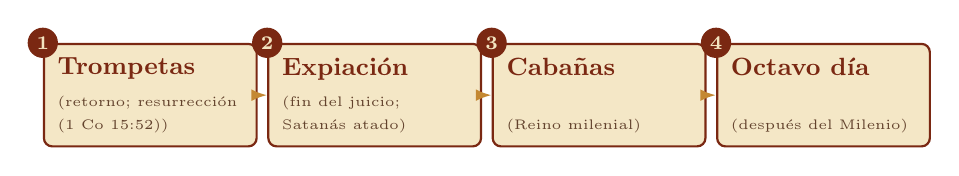
\begin{tikzpicture}[font=\scriptsize]
 \foreach \x/\n/\t/\r in {0/1/{Trompetas}/{retorno; resurrección (1 Co 15:52)}, 2.85/2/{Expiación}/{fin del juicio; Satanás atado}, 5.7/3/{Cabañas}/{Reino milenial}, 8.55/4/{Octavo día}/{después del Milenio}}{
  \node[caja,anchor=north] (b\n) at (\x,0) {\parbox[t][0.95cm][t]{2.35cm}{\RaggedRight
    {\small\textbf{\textcolor{tierraroja}{\t}}}\par\vfill{\tiny\color{sepia}(\r)}}};
  \node[circle,fill=tierraroja,text=papiro,font=\scriptsize\bfseries,inner sep=1.6pt] at (b\n.north west) {\n};}
 \foreach \a/\b in {1/2,2/3,3/4}\draw[-{Latex[length=2mm]},mostaza!80!tierraroja,line width=0.9pt] (b\a.east) -- (b\b.west);
\end{tikzpicture}\par
\scriptsize ``No se levantarán los malos en el juicio, ni los pecadores en la congregación de los justos'' (Sal 1:5).
\end{frame}

\begin{frame}{Azazel: el instigador}
\begin{columns}[t,onlytextwidth]
\begin{column}{0.50\textwidth}
\begin{cita}[fontupper=\scriptsize\itshape]El que hubiere llevado el macho cabrío a Azazel, lavará sus vestidos, lavará también con agua su cuerpo, y después entrará en el campamento.\fuente{(Lv 16:26)}\end{cita}
\scriptsize Para la serie, el macho no puede ser Cristo, porque \destacar{nuestro Señor nunca fue contaminado}. Figura a Satanás, ``el inductor de los pecados de la humanidad'', atado por mil años (Ap 20:1--3).
\end{column}
\begin{column}{0.48\textwidth}\scriptsize
\destacar{Así juzga Dios}
\begin{itemize}
\item Gn 3:14--15: la sentencia empieza por la serpiente; el instigador ``también debió comparecer''.
\item 1~P 3:19; Jud 6: detrás de la corrupción de Noé, los ``espíritus encarcelados'', ángeles ``bajo oscuridad'' para el juicio del gran día.
\item Iglesia de Dios Unida (2011): el día elimina ``la causa principal del pecado''.
\end{itemize}
\end{column}
\end{columns}
\end{frame}

\begin{frame}{Las fiestas, reloj profético}
\begin{columns}[t,onlytextwidth]
\begin{column}{0.49\textwidth}\scriptsize
\destacar{Mis presentaciones anteriores (\emph{Yom Kippur B} y \emph{M})}
\begin{itemize}
\item Lv 23:2: \heb{מוֹעֲדֵי יְהוָה}, proclamados \heb{מִקְרָאֵי קֹדֶשׁ}.
\item LXX: \emph{moadim} = \grc{καιροί} (Gn 1:14; Lv 23:4; Nm 9:3; Sal 104:19 [103:19]).
\item Pablo: ``los tiempos y las ocasiones'' (\grc{καιρῶν}, 1~Ts 5:1; Ef 1:10); Col 2:16--17.
\item Mi conclusión entonces: Pablo estructura los tiempos futuros por las fiestas.
\end{itemize}
\end{column}
\begin{column}{0.49\textwidth}
\begin{tcolorbox}[colback=mostaza!12,colframe=mostaza!80!tierraroja,boxrule=0.6pt,arc=2pt,fontupper=\scriptsize,title={\scriptsize Precisión},coltitle=caferojizo,colbacktitle=mostaza!35]
\emph{Mikrá} (\heb{קָרָא}) es ``convocación'' y ``lectura'' (Neh 8:8); ``ensayo'' es analogía, no significado. El vínculo \emph{moed} $\rightarrow$ \grc{καιρός} es real; su uso en 1~Ts 5:1 para las fiestas es inferencia posible. Los setenta traductores en celdas separadas: leyenda (Carta de Aristeas; Filón; b. Meguilá 9a).
\end{tcolorbox}
\end{column}
\end{columns}
\end{frame}

\begin{frame}{El día de la ira}
\begin{columns}[t,onlytextwidth]
\begin{column}{0.52\textwidth}
\begin{cita}[fontupper=\scriptsize\itshape]He pisado yo solo el lagar\ldots{} y su sangre salpicó mis vestidos\ldots{} Porque el día de la venganza está en mi corazón, y el año de mis redimidos ha llegado.\fuente{(Is 63:3--4)}\end{cita}
\scriptsize ``El año de mis redimidos'' (\heb{שְׁנַת גְּאוּלַי}) $\rightarrow$ Jubileo (Lv 25:8--17) y \emph{goel} (Lv 25:25; Rut 3--4; Nm 35; Job 19:25 ---mis láminas decían 9:25---).
\end{column}
\begin{column}{0.46\textwidth}\scriptsize
\begin{itemize}
\item Profetas: Sal 110:5; Is 13:9; Sof 1:7, 14--16 (``día de ira aquel día'').
\item Apóstoles: Ro 2:5; Ap 14:10, 19--20; 16:1, 19; 19:13.
\item \destacar{Ap 15:8}: ``el templo se llenó de humo\ldots{} y nadie podía entrar'' $\leftrightarrow$ Lv 16:13, 17.
\item Refugio: ``me esconderá en su tabernáculo en el día del mal'' (Sal 27:5).
\end{itemize}
\end{column}
\end{columns}
\end{frame}

\begin{frame}{El cuadro de las dos escenas}
\centering
\resizebox{0.93\linewidth}{!}{%
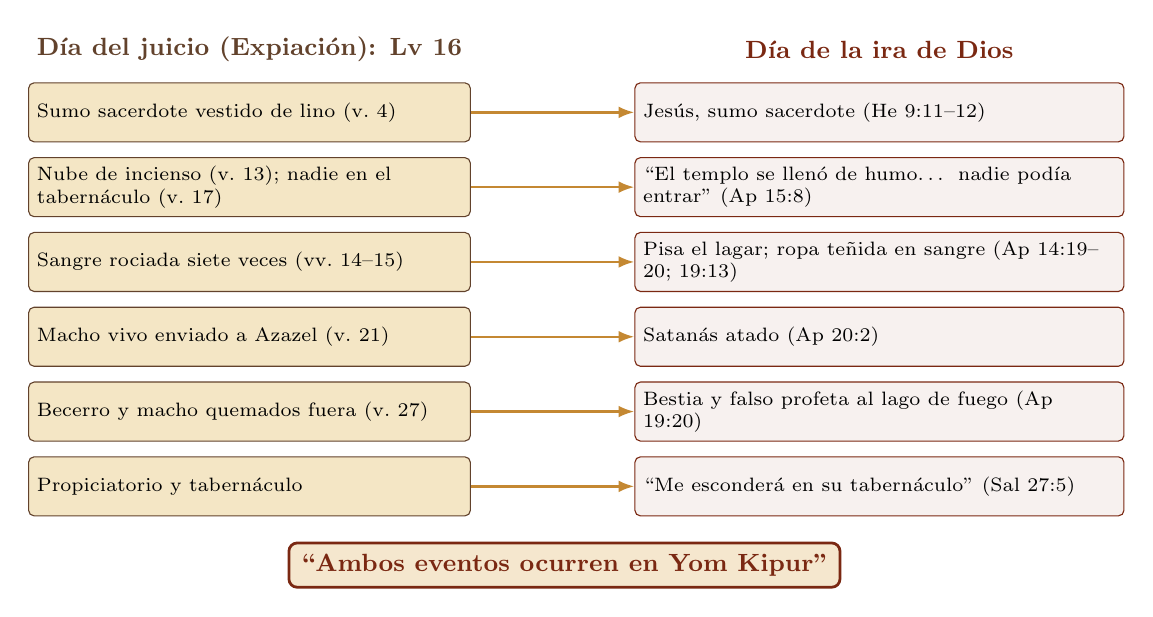
\begin{tikzpicture}[font=\scriptsize,
  l/.style={draw=sepia,fill=papiro,fill opacity=0.92,text opacity=1,rounded corners=2pt,text width=5.4cm,align=left,inner sep=3pt,minimum height=0.75cm},
  r/.style={draw=tierraroja,fill=tierraroja!7,fill opacity=0.92,text opacity=1,rounded corners=2pt,text width=6.0cm,align=left,inner sep=3pt,minimum height=0.75cm},
  fl/.style={-{Latex[length=2mm]},mostaza!80!tierraroja,line width=0.9pt}]
 \node[font=\small\bfseries,text=sepia] at (0,0.8) {Día del juicio (Expiación): Lv 16};
 \node[font=\small\bfseries,text=tierraroja] at (8,0.8) {Día de la ira de Dios};
 \foreach \y/\a/\b in {
   0/{Sumo sacerdote vestido de lino (v.~4)}/{Jesús, sumo sacerdote (He 9:11--12)},
   -0.95/{Nube de incienso (v.~13); nadie en el tabernáculo (v.~17)}/{``El templo se llenó de humo\ldots{} nadie podía entrar'' (Ap 15:8)},
   -1.9/{Sangre rociada siete veces (vv.~14--15)}/{Pisa el lagar; ropa teñida en sangre (Ap 14:19--20; 19:13)},
   -2.85/{Macho vivo enviado a Azazel (v.~21)}/{Satanás atado (Ap 20:2)},
   -3.8/{Becerro y macho quemados fuera (v.~27)}/{Bestia y falso profeta al lago de fuego (Ap 19:20)},
   -4.75/{Propiciatorio y tabernáculo}/{``Me esconderá en su tabernáculo'' (Sal 27:5)}}{
   \node[l] (a) at (0,\y) {\a}; \node[r] (b) at (8,\y) {\b}; \draw[fl] (a) -- (b);}
 \node[draw=tierraroja,line width=1pt,fill=mostaza!25,rounded corners=3pt,font=\small\bfseries,text=tierraroja,inner sep=4pt] at (4,-5.75) {``Ambos eventos ocurren en Yom Kipur''};
\end{tikzpicture}}\par\smallskip
\precision{lectura tipológica mía. He 13:11--12 aplica la quema fuera del campamento a Jesús, no a la bestia; el paralelo Ap 15:8 / Lv 16:13, 17 es estrecho.}
\end{frame}

\begin{frame}{Precisiones a la lectura de la serie}
\scriptsize
\begin{itemize}\setlength{\itemsep}{2pt}
\item \textbf{Tipología}: el vínculo con el fin del juicio del desierto no es explícito. Tiene apoyos (Nm 14:20, 34; Jos 5:9), pero Israel cruzó el Jordán ``el diez del mes \emph{primero}'' (Jos 4:19), de modo que la correspondencia es de sentido y no de fecha.
\item \textbf{Otras memorias}: Jubileos 34 (José); los rabinos, las segundas tablas tras el becerro de oro (Seder Olam Rabá 6; b. Taanit 30b).
\item \textbf{Lv 16:26}: también se lava quien quema el macho ``para el \SENOR'' (16:28; cf. Nm 19:7--10). El argumento más fuerte es el paralelo \emph{laYHWH} / \emph{laAzazel} y que el macho nunca se ofrece.
\item \textbf{Judas y 1~Enoc}: 1~En 10:4--6 ata a Azazel en la oscuridad ``hasta el gran día del juicio''; Judas cita 1~Enoc (v. 14). Eco favorable a la serie.
\item \textbf{Citas}: el texto de memoria es Ro 6:22--23 (no 6:12--13); el ayuno, Hch 27:9 (no 28:9). ``Pontífice'' es voz de la RV1909.
\item \textbf{Hebreos}: anónimo; atribuido a Pablo por la tradición oriental (Attridge, 1989; Lane, 1991). Apoyo paulino: Ro 3:25; 8:34.
\end{itemize}
\end{frame}

% ==================================================================
\section{Mesías}

\begin{frame}{Melquisedec, rey de justicia}
\begin{columns}[t,onlytextwidth]
\begin{column}{0.50\textwidth}
\begin{cita}[fontupper=\scriptsize\itshape]Entonces Melquisedec, rey de Salem y sacerdote del Dios Altísimo, sacó pan y vino\ldots\fuente{(Gn 14:18)}\end{cita}
\begin{cita}[fontupper=\scriptsize\itshape]Juró \SENOR, y no se arrepentirá: Tú eres sacerdote para siempre según el orden de Melquisedec.\fuente{(Sal 110:4)}\end{cita}
\end{column}
\begin{column}{0.48\textwidth}\scriptsize
\begin{itemize}
\item Primer \heb{כֹּהֵן} de la Biblia; \heb{מַלְכִּי־צֶדֶק}: ``rey de justicia''; Salem: ``paz'' (He 7:2).
\item Pan, vino, bendición y diezmo del botín (Gn 14:17--20).
\item El rey davídico recibe un sacerdocio \destacar{anterior a Aarón y sin término}.
\end{itemize}
\precision{En mi presentación propuse que Abram mató a un pariente (Elam, hijo de Sem, Gn 10:22) y Melquisedec hizo la paz: hipótesis. Melquisedec = Sem es tradición judía (Targumim; b. Nedarim 32b).}
\end{column}
\end{columns}
\end{frame}

\begin{frame}{Precisión: Sal 110 y los ``134''}
\small
\begin{itemize}
\item Una lámina afirma que el TM ``ha sido alterado 134 veces''.
\item La tradición masorética enumera \destacar{134 lugares} en que los escribas habrían escrito \heb{אֲדֹנָי} donde estaba el tetragrama, por reverencia al Nombre (Ginsburg, 1897).
\item Es una noticia sobre la escritura del Nombre, \destacar{no una prueba de alteración} del sentido.
\item Sal 110:1 distingue \heb{נְאֻם יְהוָה} (``dijo el \SENOR'') y \heb{לַאדֹנִי} (``a mi señor''); LXX \grc{εἶπεν ὁ κύριος τῷ κυρίῳ μου}; Mt 22:44.
\end{itemize}
\end{frame}

\begin{frame}{``Según el orden'': \grc{τάξις}}
\begin{columns}[t,onlytextwidth]
\begin{column}{0.49\textwidth}\scriptsize
\begin{itemize}
\item \grc{τάξις}: orden, secuencia, turno. Zacarías ofició ``según el orden de su clase'' (Lc 1:8), la de Abías (1~Cr 24:3--10).
\item Cristo, sumo sacerdote por \destacar{juramento} (He 7:20--28) y ``según el poder de una vida indestructible'' (7:16).
\item \emph{Tsédeq} / \grc{δικαιοσύνη}: Melquisedec, Sadoc (2~S 8:17), Cristo ``justo'' (1~Jn 2:1, 29).
\end{itemize}
\end{column}
\begin{column}{0.49\textwidth}\scriptsize
\destacar{La ``transferencia del orden'' (mi lectura)}
\begin{itemize}
\item Juan, de linaje sacerdotal, bautiza: ``así conviene que cumplamos toda justicia'' (Mt 3:15).
\item Caifás ``rasgó sus vestiduras'' (Mt 26:65; prohibido: Lv 10:6; 21:10); la túnica de Jesús, ``sin costura'' (Jn 19:23).
\item ``nos hizo reyes y sacerdotes'' (Ap 1:6; 5:10).
\end{itemize}
\precision{lectura tipológica; Juan cita el Sal 22 como clave de la túnica (Jn 19:24). ``Noé, el octavo'' (2~P 2:5) suele leerse, con la RVR1960, ``con otras siete personas'' (cf. 1~P 3:20).}
\end{column}
\end{columns}
\end{frame}

\begin{frame}{11QMelquisedec}
\scriptsize
\begin{itemize}
\item Combina Lv 25 (Jubileo), Dt 15:2 (remisión) e Is 61:1: Melquisedec proclama \destacar{liberación} de las iniquidades.
\item ``el día de las expiaciones es el final del décimo jubileo, en el que se hará expiación por todos los hijos de la luz'' (11Q13 II 7--8).
\item Is 61:2 reescrito: \destacar{``el año del favor de Melquisedec''} (II 9).
\item Ejecuta el juicio de Dios contra \destacar{Belial} y los espíritus de su lote (II 13).
\end{itemize}
\begin{tcolorbox}[colback=mostaza!12,colframe=mostaza!80!tierraroja,boxrule=0.6pt,arc=2pt,fontupper=\scriptsize]
Jubileo + Yom Kipur + liberación + juicio contra el adversario: un paralelo antiguo de la lectura de la serie. Texto fragmentario, con reconstrucciones (García Martínez, 1992; Bergsma, 2007).
\end{tcolorbox}
\end{frame}

\begin{frame}{He 9: el Yom Kipur del Mesías}
\begin{cita}[fontupper=\scriptsize\itshape]\ldots{}y no por sangre de machos cabríos ni de becerros, sino por su propia sangre, entró una vez para siempre en el Lugar Santísimo, habiendo obtenido eterna redención.\fuente{(He 9:12)}\end{cita}
\centering
\resizebox{0.92\linewidth}{!}{%
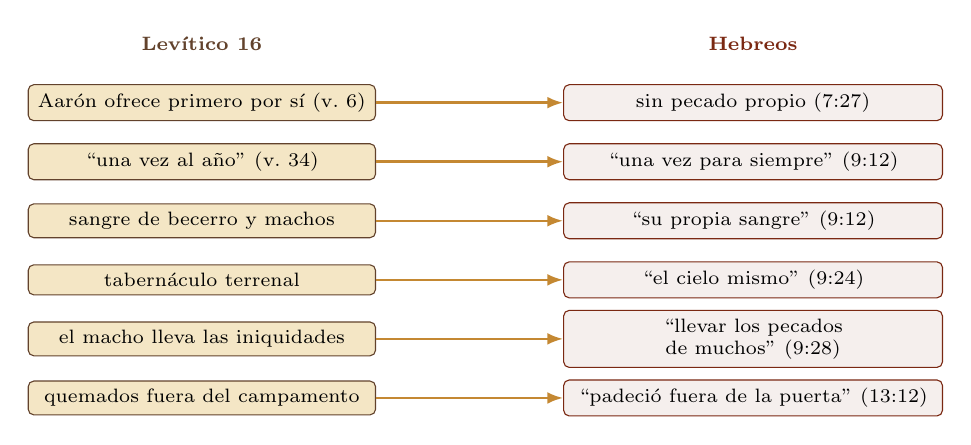
\begin{tikzpicture}[font=\scriptsize,
  l/.style={draw=sepia,fill=papiro,fill opacity=0.92,text opacity=1,rounded corners=2pt,text width=4.2cm,align=center,inner sep=3pt},
  r/.style={draw=tierraroja,fill=tierraroja!8,fill opacity=0.92,text opacity=1,rounded corners=2pt,text width=4.6cm,align=center,inner sep=3pt},
  fl/.style={-{Latex[length=2mm]},mostaza!80!tierraroja,line width=0.9pt}]
 \node[font=\scriptsize\bfseries,text=sepia] at (0,0.75) {Levítico 16};
 \node[font=\scriptsize\bfseries,text=tierraroja] at (7,0.75) {Hebreos};
 \foreach \y/\a/\b in {0/{Aarón ofrece primero por sí (v.~6)}/{sin pecado propio (7:27)},
                      -0.75/{``una vez al año'' (v.~34)}/{``una vez para siempre'' (9:12)},
                      -1.5/{sangre de becerro y machos}/{``su propia sangre'' (9:12)},
                      -2.25/{tabernáculo terrenal}/{``el cielo mismo'' (9:24)},
                      -3.0/{el macho lleva las iniquidades}/{``llevar los pecados de muchos'' (9:28)},
                      -3.75/{quemados fuera del campamento}/{``padeció fuera de la puerta'' (13:12)}}{
   \node[l] (a) at (0,\y) {\a}; \node[r] (b) at (7,\y) {\b}; \draw[fl] (a) -- (b);}
\end{tikzpicture}}
\end{frame}

\begin{frame}{``Aparecerá por segunda vez''}
\fotolado{panel_he9_28.jpg}{Elaboración propia: He 9:28b en escritura uncial (texto NA28).}
\begin{columns}[c,onlytextwidth]
\begin{column}{0.57\textwidth}
\begin{cita}\ldots{}así también Cristo fue ofrecido una sola vez para llevar los pecados de muchos; y aparecerá por segunda vez, sin relación con el pecado, para salvar a los que le esperan.\fuente{(He 9:28)}\end{cita}
\scriptsize Israel esperaba en el atrio la \destacar{salida} del sumo sacerdote (Lv 16:17, 24; Si 50:5). \grc{ἐκ δευτέρου\ldots{} ὀφθήσεται τοῖς αὐτὸν ἀπεκδεχομένοις}: la Iglesia vive \destacar{entre la entrada y la salida} de su sumo sacerdote. Es la base más clara de la lectura de la serie.
\end{column}
\begin{column}{0.41\textwidth}\end{column}
\end{columns}
\end{frame}

\begin{frame}{Entrada y salida}
\centering
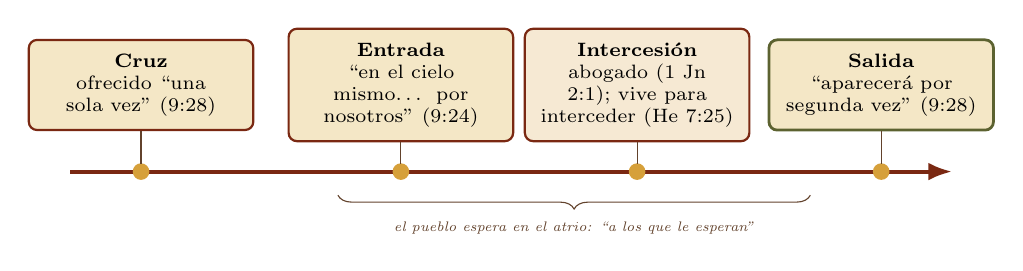
\begin{tikzpicture}[font=\scriptsize]
 \draw[line width=1.4pt,tierraroja,-{Latex[length=3mm]}] (0,0) -- (11.2,0);
 \node[caja,text width=2.5cm,align=center] (c) at (0.9,1.1) {\textbf{Cruz}\\ ofrecido ``una sola vez'' (9:28)};
 \node[caja,text width=2.5cm,align=center] (e) at (4.2,1.1) {\textbf{Entrada}\\ ``en el cielo mismo\ldots{} por nosotros'' (9:24)};
 \node[caja,text width=2.5cm,align=center,fill=mostaza!25] (i) at (7.2,1.1) {\textbf{Intercesión}\\ abogado (1~Jn 2:1); vive para interceder (He 7:25)};
 \node[caja,text width=2.5cm,align=center,draw=oliva,line width=1pt] (s) at (10.3,1.1) {\textbf{Salida}\\ ``aparecerá por segunda vez'' (9:28)};
 \foreach \n/\x in {c/0.9,e/4.2,i/7.2,s/10.3}{\fill[mostaza] (\x,0) circle (3pt); \draw[sepia] (\n.south) -- (\x,0.1);}
 \draw[decorate,decoration={brace,amplitude=5pt,mirror},sepia] (3.4,-0.3) -- (9.4,-0.3) node[midway,below=6pt,font=\tiny\itshape,align=center]{el pueblo espera en el atrio: ``a los que le esperan''};
\end{tikzpicture}\par\medskip
\small\RaggedRight El velo abierto: ``camino nuevo y vivo que él nos abrió a través del velo, esto es, de su carne'' (He 10:20; Mt 27:51). ``Hoy con Yeshúa tenemos entrada al Lugar Santísimo'' (así lo resumí en mis láminas).
\end{frame}

\begin{frame}{Pablo, Juan, Lucas y el Apocalipsis}
\scriptsize
\begin{columns}[t,onlytextwidth]
\begin{column}{0.49\textwidth}
\begin{itemize}
\item \textbf{Ro 3:25}: Cristo, \grc{ἱλαστήριον}, ``puesto'' a la vista: lo oculto tras el velo, expuesto en la cruz.
\item \textbf{2~Co 5:21}: ``lo hizo pecado'' (¿o ``sacrificio por el pecado''? \emph{jatat}, LXX Lv 4:21).
\item \textbf{1~Jn 2:2}: ``él es la propiciación\ldots{} por los de todo el mundo''.
\end{itemize}
\end{column}
\begin{column}{0.49\textwidth}
\begin{itemize}
\item \textbf{Hch 27:9}: ``por haber pasado ya el ayuno'' (\grc{τὴν νηστείαν}).
\item \textbf{Ap 8:3--4}: incensario de oro y oraciones de los santos.
\item \textbf{Ap 11:19}: ``el arca de su pacto se veía en el templo''.
\item \textbf{Ap 20:1--3}: la serpiente antigua, atada y sellada en el abismo.
\end{itemize}
\end{column}
\end{columns}\par\medskip
\precision{ecos en la pasión que recogí en mis presentaciones (suertes, Sal 22:18 [22:19]; Barrabás, Orígenes, \emph{Hom. Lev.} 10.2; manto escarlata, Bernabé 7): ecos posibles, no cumplimientos declarados.}
\end{frame}

% ==================================================================
\section{Tradición}

\begin{frame}{El servicio según la Misná}
\scriptsize
\begin{columns}[t,onlytextwidth]
\begin{column}{0.49\textwidth}
\begin{itemize}
\item Siete días de separación y práctica (Yomá 1:1--3).
\item \destacar{Tres confesiones}: por sí y su casa (3:8), por los sacerdotes (4:2), por Israel sobre el macho vivo (6:2).
\item El Nombre pronunciado; el pueblo responde: ``Bendito sea el nombre de la gloria de su reino por siempre jamás'' (6:2).
\end{itemize}
\end{column}
\begin{column}{0.49\textwidth}
\begin{itemize}
\item La urna de las suertes (3:9; 4:1); la \destacar{cinta escarlata} (4:2; 6:6) que blanqueaba (6:8; Is 1:18).
\item Diez puestos hasta el despeñadero (6:4).
\item Oración breve ``para no atemorizar a Israel'' (5:1); fiesta al salir en paz (7:4).
\end{itemize}
\end{column}
\end{columns}\par\medskip
\precision{tradición rabínica, compilada hacia el 200 e.\,c. El Nombre diez veces: \emph{baraita} en b. Yomá 39b.}
\end{frame}

\begin{frame}{Del templo a la sinagoga}
\begin{cita}[fontupper=\scriptsize\itshape]Las transgresiones entre el hombre y Dios, el día de las expiaciones las expía; las transgresiones entre el hombre y su prójimo, el día de las expiaciones no las expía hasta que haya apaciguado a su prójimo.\fuente{(Misná Yomá 8:9; cf. Mt 5:23--24)}\end{cita}
\scriptsize
\begin{itemize}\setlength{\itemsep}{1pt}
\item Diez días de arrepentimiento; libros abiertos (b. Rosh haShaná 16b).
\item Lecturas: Lv 16; Is 57:14--58:14 (``¿No es más bien el ayuno que yo escogí\ldots?'', 58:6); Jonás en la tarde (b. Meguilá 31a).
\item \emph{Neilá}; \emph{Kol Nidré} (época gueónica); \emph{kaparot} (medieval).
\end{itemize}
\precision{las ``tres trompetas'' (primera, última, gran trompeta) son enseñanza mesiánica popular; lo bíblico es el shofar del Jubileo en Yom Kipur (Lv 25:9).}
\end{frame}

% ==================================================================
\section{Discusión}

\begin{frame}{Lecturas de Azazel}
\tiny\renewcommand{\arraystretch}{1.15}
\begin{tabular}{@{}L{2.4cm}L{3.6cm}L{3.5cm}L{2.4cm}@{}}
\toprule
\textbf{Lectura} & \textbf{Argumento} & \textbf{Autores} & \textbf{Dificultad} \\ \midrule
Macho que se va & \emph{ez ozel} & LXX; Vulgata; Tyndale & ``enviarlo \emph{a} Azazel'' \\
Lugar escarpado & destino del animal & Misná; Talmud; Targum; Driver (1956) & ya dice ``al desierto'' \\
Ser demoníaco & \emph{laYHWH} / \emph{laAzazel}; Lv 17:7 & 1~Enoc; Milgrom (1991); Levine (1989); Hartley (1992); Wright (1987) & no se le ofrece nada \\
Satanás, instigador & Lv 16:26; Gn 3; Ap 20 & Keil y Delitzsch (1864); White (1888); Iglesia de Dios Unida (2011); documento de referencia & el NT no nombra a Azazel \\
Cristo que quita el pecado & un sacrificio en dos animales; Is 53; He 9:28 & Bernabé 7; M. Henry; lectura reformada & no se ofrece; su conductor queda impuro \\
\bottomrule
\end{tabular}\par\medskip
\scriptsize Mis presentaciones anteriores recogen dos de ellas: ``los dos carneros\ldots{} un signo del Mesías'' y ``Azazel\ldots{} imagen de Satanás''.
\end{frame}

\begin{frame}{Balance}
\small
\begin{enumerate}\setlength{\itemsep}{2pt}
\item El NT \destacar{nunca nombra a Azazel}; sus alusiones se concentran en el sumo sacerdote, la sangre, el velo y el santuario.
\item Cuando dice que Cristo ``lleva'' el pecado, usa Is 53, el lenguaje de Lv 16:22: \destacar{apoyo verbal} para la lectura cristológica.
\item \emph{laYHWH} / \emph{laAzazel}, 1~Enoc (conocido por Judas), Zac 3 y 11QMelquisedec: \destacar{apoyo histórico} para la lectura de la serie.
\item Lv 16 dice que el macho lleva ``las iniquidades \emph{de ellos}''; la culpa del instigador se alcanza por Gn 3 y Ap 20, esto es, por \destacar{la Biblia que interpreta la Biblia}.
\end{enumerate}
\scriptsize Pueden convivir: Cristo carga y quita el pecado (He 9:28); el instigador es juzgado y apartado (Ro 16:20; Ap 20:1--3).
\end{frame}

\begin{frame}{¿Qué purifica? ¿Qué juicio?}
\begin{columns}[t,onlytextwidth]
\begin{column}{0.49\textwidth}\scriptsize
\destacar{El mecanismo}
\begin{itemize}
\item Milgrom (1991): el pecado contamina el santuario a distancia; el día limpia todas sus zonas.
\item Gane (2005): segunda fase; Dios purga su morada de las faltas ya perdonadas.
\item Wenham (1979); Hartley (1992): purificación cultual y moral.
\end{itemize}
\end{column}
\begin{column}{0.49\textwidth}\scriptsize
\destacar{El juicio}
\begin{itemize}
\item Serie: juicio en curso sobre la casa de Dios (1~P 4:17), concluido con la salida del Sumo Pontífice.
\item Lectura evangélica: ``ninguna condenación hay'' (Ro 8:1), aunque todos comparecerán (2~Co 5:10).
\item En 1~P 4:12--19 el juicio \destacar{ya comenzó}: el sufrimiento que purifica.
\end{itemize}
\end{column}
\end{columns}
\end{frame}

% ==================================================================
\section{Síntesis}

\begin{frame}{Definición}
\begin{tcolorbox}[colback=papiro,colframe=tierraroja,boxrule=1pt,arc=3pt,fontupper=\scriptsize]
\textbf{Yom haKipurim}: convocación santa del 10 del mes séptimo, \emph{shabat shabatón} y ayuno, en que el sumo sacerdote entraba una vez al año tras el velo para purificar el santuario, la tienda y el altar, y enviaba al desierto el macho vivo cargado con las iniquidades confesadas, para que Dios siguiera habitando ``en medio de sus impurezas'' (Lv 16:16) y el pueblo fuera limpio ``delante de \SENOR'' (16:30). Cristo es el sumo sacerdote que entró ``una vez para siempre'' y ``aparecerá por segunda vez'' (He 9:12, 28). Para la serie, el día anuncia el fin del juicio a la casa de Dios y el juicio de Satanás (Ap 20:1--3).
\end{tcolorbox}
\tiny\renewcommand{\arraystretch}{1.1}
\begin{tabular}{@{}L{2.0cm}L{9.6cm}@{}}
\toprule
Histórica & del desierto al Segundo Templo; el día sobrevive al año 70 \\
Filológica & \emph{kipper}; \emph{kapóret} $\rightarrow$ \grc{ἱλαστήριον}; tres palabras del pecado; \emph{nasá avón} \\
Textual & LXX: Azazel = alejamiento, \grc{ἄφεσις}; Dn 9:24; Ro 3:25; He 9:4 \\
Literaria & Lv 16 en el centro; de dentro hacia fuera; dos machos, un acto \\
Serie y NT & Sumo Pontífice; entrada y salida; Azazel y el instigador \\
\bottomrule
\end{tabular}
\end{frame}

% ==================================================================
\section{Reflexión}

\begin{frame}{Para la reflexión}
\small
\begin{enumerate}\setlength{\itemsep}{3pt}
\item Si el pecado afecta el lugar donde Dios habita (Lv 16:16; 1~Co 3:16--17), ¿cómo cambia la manera de confesarlo?
\item ¿Distingo en mi confesión lo torcido (\emph{avón}), lo rebelde (\emph{pésha}) y lo fallido (\emph{jatat})?
\item ¿Qué reconciliación con el prójimo debería preceder a mi ayuno (Misná Yomá 8:9; Mt 5:23--24)?
\item ¿Qué ``yugo'' concreto puede desatar mi ayuno (Is 58:6)?
\item ¿Cómo vivo la espera de la salida de mi sumo sacerdote (He 9:28): con temor, con indiferencia o con certeza?
\item ``Entonces veremos cara a cara'' (1~Co 13:12): ¿es ese encuentro el horizonte de mi vida?
\end{enumerate}
\end{frame}

% ==================================================================
\section{Glosario}

\begin{frame}{Glosario}
\scriptsize
\begin{columns}[t,onlytextwidth]
\begin{column}{0.49\textwidth}
\begin{description}\setlength{\itemsep}{1pt}
\item[Azazel] (\heb{עֲזָאזֵל}) destinatario del segundo macho (Lv 16:8).
\item[\emph{Derór}] (\heb{דְּרוֹר}) libertad del Jubileo (Lv 25:10).
\item[\emph{Goral}] (\heb{גּוֹרָל}) suerte.
\item[\emph{Hilastérion}] (\grc{ἱλαστήριον}) propiciatorio; Ro 3:25.
\item[\emph{Hilasmós}] (\grc{ἱλασμός}) propiciación (1~Jn 2:2).
\item[\emph{Inui néfesh}] (\heb{עִנּוּי נֶפֶשׁ}) ayuno.
\item[\emph{Jatat}] (\heb{חַטָּאת}) pecado; ofrenda por el pecado.
\item[\emph{Kapóret}] (\heb{כַּפֹּרֶת}) tapa del arca.
\end{description}
\end{column}
\begin{column}{0.49\textwidth}
\begin{description}\setlength{\itemsep}{1pt}
\item[\emph{Karet}] (\heb{כָּרֵת}) ser cortado del pueblo.
\item[\emph{Ketóret}] (\heb{קְטֹרֶת}) incienso.
\item[\emph{Kipper}] (\heb{כִּפֶּר}) expiar: cubrir, rescatar, purgar.
\item[\emph{Kipurim}] (\heb{כִּפֻּרִים}) la expiación (plural).
\item[\emph{Nasá avón}] (\heb{נָשָׂא עָוֺן}) llevar la iniquidad.
\item[\emph{Neilá}] (\heb{נְעִילָה}) oración de cierre.
\item[\emph{Parójet}] (\heb{פָּרֹכֶת}) el velo.
\item[\emph{Shabat shabatón}] (\heb{שַׁבַּת שַׁבָּתוֹן}) reposo absoluto.
\end{description}
\end{column}
\end{columns}
\end{frame}

% ==================================================================
\section{Referencias}

\begin{frame}{Referencias (1)}
\tiny
\refapa{Las citas bíblicas son de la Reina-Valera 1960 (Sociedades Bíblicas en América Latina, 1960), con \SENOR{} donde dice ``Jehová''; hebreo según la BHS (Elliger y Rudolph, 1997); griego según NA28 (2012) y Rahlfs y Hanhart (2006).}
\refapa{Attridge, H.~W. (1989). \emph{The epistle to the Hebrews}. Fortress.}
\refapa{Bergsma, J.~S. (2007). \emph{The Jubilee from Leviticus to Qumran}. Brill.}
\refapa{Brown, F., Driver, S.~R., \& Briggs, C.~A. (1906). \emph{A Hebrew and English lexicon of the Old Testament}. Clarendon.}
\refapa{Danby, H. (Trad.). (1933). \emph{The Mishnah}. Oxford University Press.}
\refapa{Dodd, C.~H. (1935). \emph{The Bible and the Greeks}. Hodder \& Stoughton.}
\refapa{Douglas, M. (1999). \emph{Leviticus as literature}. Oxford University Press.}
\refapa{Driver, G.~R. (1956). Three technical terms in the Pentateuch. \emph{Journal of Semitic Studies, 1}(2), 97--105.}
\refapa{Dunn, J.~D.~G. (1998). \emph{The theology of Paul the apostle}. Eerdmans.}
\refapa{Gane, R. (2005). \emph{Cult and character}. Eisenbrauns.}
\refapa{García Martínez, F. (1992). \emph{Textos de Qumrán}. Trotta.}
\refapa{Ginsburg, C.~D. (1897). \emph{Introduction to the Massoretico-critical edition of the Hebrew Bible}. Trinitarian Bible Society.}
\refapa{Hartley, J.~E. (1992). \emph{Leviticus} (WBC 4). Word.}
\refapa{Hayward, C.~T.~R. (1996). \emph{The Jewish temple: A non-biblical sourcebook}. Routledge.}
\refapa{Henry, M. (1999). \emph{Comentario bíblico de Matthew Henry}. CLIE.}
\end{frame}

\begin{frame}{Referencias (2)}
\tiny
\refapa{Holmes, M.~W. (Ed.). (2007). \emph{The Apostolic Fathers} (3.ª ed.). Baker Academic.}
\refapa{Iglesia de Dios Unida. (2011). \emph{Las fiestas santas de Dios: esperanza segura para toda la humanidad}.}
\refapa{Keil, C.~F., \& Delitzsch, F. (1996). \emph{Commentary on the Old Testament: The Pentateuch}. Hendrickson. (Original publicado en 1864)}
\refapa{Lane, W.~L. (1991). \emph{Hebrews} (WBC 47A--B). Word.}
\refapa{Levine, B.~A. (1989). \emph{Leviticus} (JPS Torah Commentary). Jewish Publication Society.}
\refapa{Milgrom, J. (1991). \emph{Leviticus 1--16} (AB 3). Doubleday.}
\refapa{Moo, D.~J. (1996). \emph{The epistle to the Romans} (NICNT). Eerdmans.}
\refapa{Morris, L. (1955). \emph{The apostolic preaching of the cross}. Tyndale Press.}
\refapa{Nickelsburg, G.~W.~E. (2001). \emph{1 Enoch 1} (Hermeneia). Fortress.}
\refapa{Sefaria. (s.~f.). \emph{Mishnah Yoma; Talmud Bavli Yoma}. https://www.sefaria.org}
\refapa{Stökl Ben Ezra, D. (2003). \emph{The impact of Yom Kippur on early Christianity}. Mohr Siebeck.}
\refapa{VanderKam, J.~C. (1998). \emph{Calendars in the Dead Sea Scrolls}. Routledge.}
\refapa{Warning, W. (1999). \emph{Literary artistry in Leviticus}. Brill.}
\refapa{Wenham, G.~J. (1979). \emph{The book of Leviticus} (NICOT). Eerdmans.}
\refapa{White, E.~G. (1888). \emph{The great controversy between Christ and Satan}. Pacific Press.}
\refapa{Wright, D.~P. (1987). \emph{The disposal of impurity}. Scholars Press.}
\end{frame}

\end{document}
